%% \cite{lynch2017modern} 
%% Copyright 2007-2024 Elsevier Ltd
%% 
%% This file is part of the 'Elsarticle Bundle'.
%% ---------------------------------------------
%% 
%% It may be distributed under the conditions of the LaTeX Project Public
%% License, either version 1.3 of this license or (at your option) any
%% later version.  The latest version of this license is in
%%    http://www.latex-project.org/lppl.txt
%% and version 1.3 or later is part of all distributions of LaTeX
%% version 1999/12/01 or later.
%% 
%% The list of all files belonging to the 'Elsarticle Bundle' is
%% given in the file `manifest.txt'.
%% 
%% Template article for Elsevier's document class `elsarticle'
%% with numbered style bibliographic references
%% SP 2008/03/01
%% $Id: elsarticle-template-num.tex 249 2024-04-06 10:51:24Z rishi $
%%
\documentclass[preprint,12pt]{elsarticle}

%% Use the option review to obtain double line spacing
%% \documentclass[authoryear,preprint,review,12pt]{elsarticle}

%% Use the options 1p,twocolumn; 3p; 3p,twocolumn; 5p; or 5p,twocolumn
%% for a journal layout:
%% \documentclass[final,1p,times]{elsarticle}
%% \documentclass[final,1p,times,twocolumn]{elsarticle}
%% \documentclass[final,3p,times]{elsarticle}
%% \documentclass[final,3p,times,twocolumn]{elsarticle}
%% \documentclass[final,5p,times]{elsarticle}
%% \documentclass[final,5p,times,twocolumn]{elsarticle}

%% For including figures, graphicx.sty has been loaded in
%% elsarticle.cls. If you prefer to use the old commands
%% please give \usepackage{epsfig}

%% The amssymb package provides various useful mathematical symbols
\usepackage{amssymb}
%% The amsmath package provides various useful equation environments.
\usepackage{amsmath}
\usepackage{hyperref}
\usepackage{booktabs}
\usepackage{multirow}
%% The amsthm package provides extended theorem environments
%% \usepackage{amsthm}

%% The lineno packages adds line numbers. Start line numbering with
%% \begin{linenumbers}, end it with \end{linenumbers}. Or switch it on
%% for the whole article with \linenumbers.
%% \usepackage{lineno}

\journal{Nuclear Physics B}

\begin{document}

\begin{frontmatter}

%% Title, authors and addresses

%% use the tnoteref command within \title for footnotes;
%% use the tnotetext command for theassociated footnote;
%% use the fnref command within \author or \affiliation for footnotes;
%% use the fntext command for theassociated footnote;
%% use the corref command within \author for corresponding author footnotes;
%% use the cortext command for theassociated footnote;
%% use the ead command for the email address,
%% and the form \ead[url] for the home page:
%% \title{Title\tnoteref{label1}}
%% \tnotetext[label1]{}
%% \author{Name\corref{cor1}\fnref{label2}}
%% \ead{email address}
%% \ead[url]{home page}
%% \fntext[label2]{}
%% \cortext[cor1]{}
%% \affiliation{organization={},
%%             addressline={},
%%             city={},
%%             postcode={},
%%             state={},
%%             country={}}
%% \fntext[label3]{}

\title{Continuous Trajectory Tracking for Non-Spherical Wrist Manipulator via Coupled-Reward-Driven Differential Inverse Kinematics}

%% use optional labels to link authors explicitly to addresses:
\author[label1]{Surya Prakash S.K}
\author[label2]{Sai Teja Majji}
\author[label2]{Darshankumar Prajapati}
\author[label2]{Jagannath Prasad Sahoo}
\author[label1]{Pushkar Kumar}
\author[label2]{Jayakumar V.K}
\author[label2]{Amit Shukla}
\affiliation[label1]{organization={School of Mechanical and Materials Engineering, IIT Mandi},
            addressline={},
            city={Mandi},
            postcode={175005},
            state={H.P},
            country={India}}

\affiliation[label2]{organization={Center for Artificial Intelligence and Robotics, IIT Mandi},
            addressline={},
            city={Mandi},
            postcode={175005},
            state={H.P},
            country={India}}

% \author{Surya Prakash S.K} %% Author name

% %% Author affiliation
% \affiliation{organization={SMME, IIT Mandi},%Department and Organization
%             addressline={Kamand}, 
%             city={Mandi},
%             postcode={175005}, 
%             state={H.P},
%             country={India}}

% \author{Surya Prakash S.K} %% Author name

% %% Author affiliation
% \affiliation{organization={SMME, IIT Mandi},%Department and Organization
%             addressline={Kamand}, 
%             city={Mandi},
%             postcode={175005}, 
%             state={H.P},
%             country={India}}
% \author{Surya Prakash S.K} %% Author name

% %% Author affiliation
% \affiliation{organization={SMME, IIT Mandi},%Department and Organization
%             addressline={Kamand}, 
%             city={Mandi},
%             postcode={175005}, 
%             state={H.P},
%             country={India}}
%% Abstract
\begin{abstract}
Continuous trajectory tracking requires differential inverse kinematics (IK) at
every control timestep; for non-spherical wrist manipulators, kinematic coupling
renders this a nonlinear problem. Existing numerical solvers that resolve
waypoints independently produce joint-space discontinuities incompatible with
real-time hardware loops. We address this through a coupled reward function,
combining a min-operator inverse-quadratic pose reward, asymmetric progress
shaping, and an exponential energy penalty, that enforces simultaneous
position-orientation convergence while suppressing velocity discontinuities,
applied here to a Proximal Policy Optimization (PPO) controller mapping a
19-dimensional observation directly to joint velocity commands. The policy is
trained in Isaac Lab on 1.5~M joint-limit-aware reachable workspace poses, with
no trajectory supervision. The proposed method achieves competitive position
and orientation accuracy in simulation against baselines spanning a numerical
IK solver, classical velocity-level controllers, and contemporary RL methods,
and outperforms the alternative RL baselines (TRPO, SAC) evaluated under an
identical reward formulation. Zero-shot sim-to-real transfer to the Kinova
Gen3 Lite at 20~Hz closed-loop frequency achieves a position RMSE of 6.3~mm
and orientation RMSE of 0.0320~rad on circular trajectory tracking, with no
degradation relative to simulation. The policy generalizes without retraining
to square, lemniscate, and 3-D Lissajous trajectories, demonstrating that a
velocity-level differential IK mapping learned purely on static pose reaching
transfers directly to arbitrary continuous trajectory tracking at deployment.
\end{abstract}

%%Graphical abstract
% \begin{graphicalabstract}

% \end{graphicalabstract}

%%Research highlights
\begin{highlights}
\item A coupled min-operator, progress, and energy-penalty reward enables stable IK.
\item Min-operator coupling prevents reward exploitation across pose objectives.
\item Policy trained only on static poses generalizes zero-shot to four trajectories.
\item Lowest smoothness index of any baseline across circle, lemniscate, Lissajous.
\end{highlights}

%% Keywords
\begin{keyword}
Differential Inverse Kinematics \sep Trajectory Tracking \sep Non-Spherical Wrist Manipulator \sep Reward Shaping \sep Reinforcement Learning \sep Sim-to-Real Transfer.

\end{keyword}

\end{frontmatter}

%% Add \usepackage{lineno} before \begin{document} and uncomment 
%% following line to enable line numbers
%% \linenumbers

%% main text
%%

%% Use \section commands to start a section
\section{Introduction}
\label{intro}
Robotic manipulators are indispensable to modern industrial automation, serving as the backbone for tasks ranging from precision assembly to complex material handling. To meet the demands of rapid advancements in the field, contemporary systems must provide not only mechanical precision but also intelligent, computationally efficient manipulation in real-time \cite{intro_1}. Traditionally, spherical wrist designs have dominated the industry due to their kinematic decoupling, which facilitates independent, closed-form analytical solutions for position and orientation \cite{intro_2}. While these designs have long been the industrial standard, they impose significant structural limitations on modern applications \cite{shah2019comparison}. The geometric constraint requiring the final three axes to intersect at a common point,  often compromises mechanical stiffness and restricts the integration of high-torque motors within compact wrist assemblies \cite{ostermeier}. Consequently, non-spherical wrist manipulators have gained prominence. By introducing offsets between the last three axes as shown in Fig.~\ref{fig:sphericalvsnonspherical}, these configurations achieve superior structural integrity and higher payload-to-weight ratios \cite{carbonari2023inverse}. However, this violation of kinematic decoupling renders analytical inverse kinematics (IK) intractable, necessitating a reliance on complex numerical or data-driven solvers. 
\begin{figure}
    \centering
    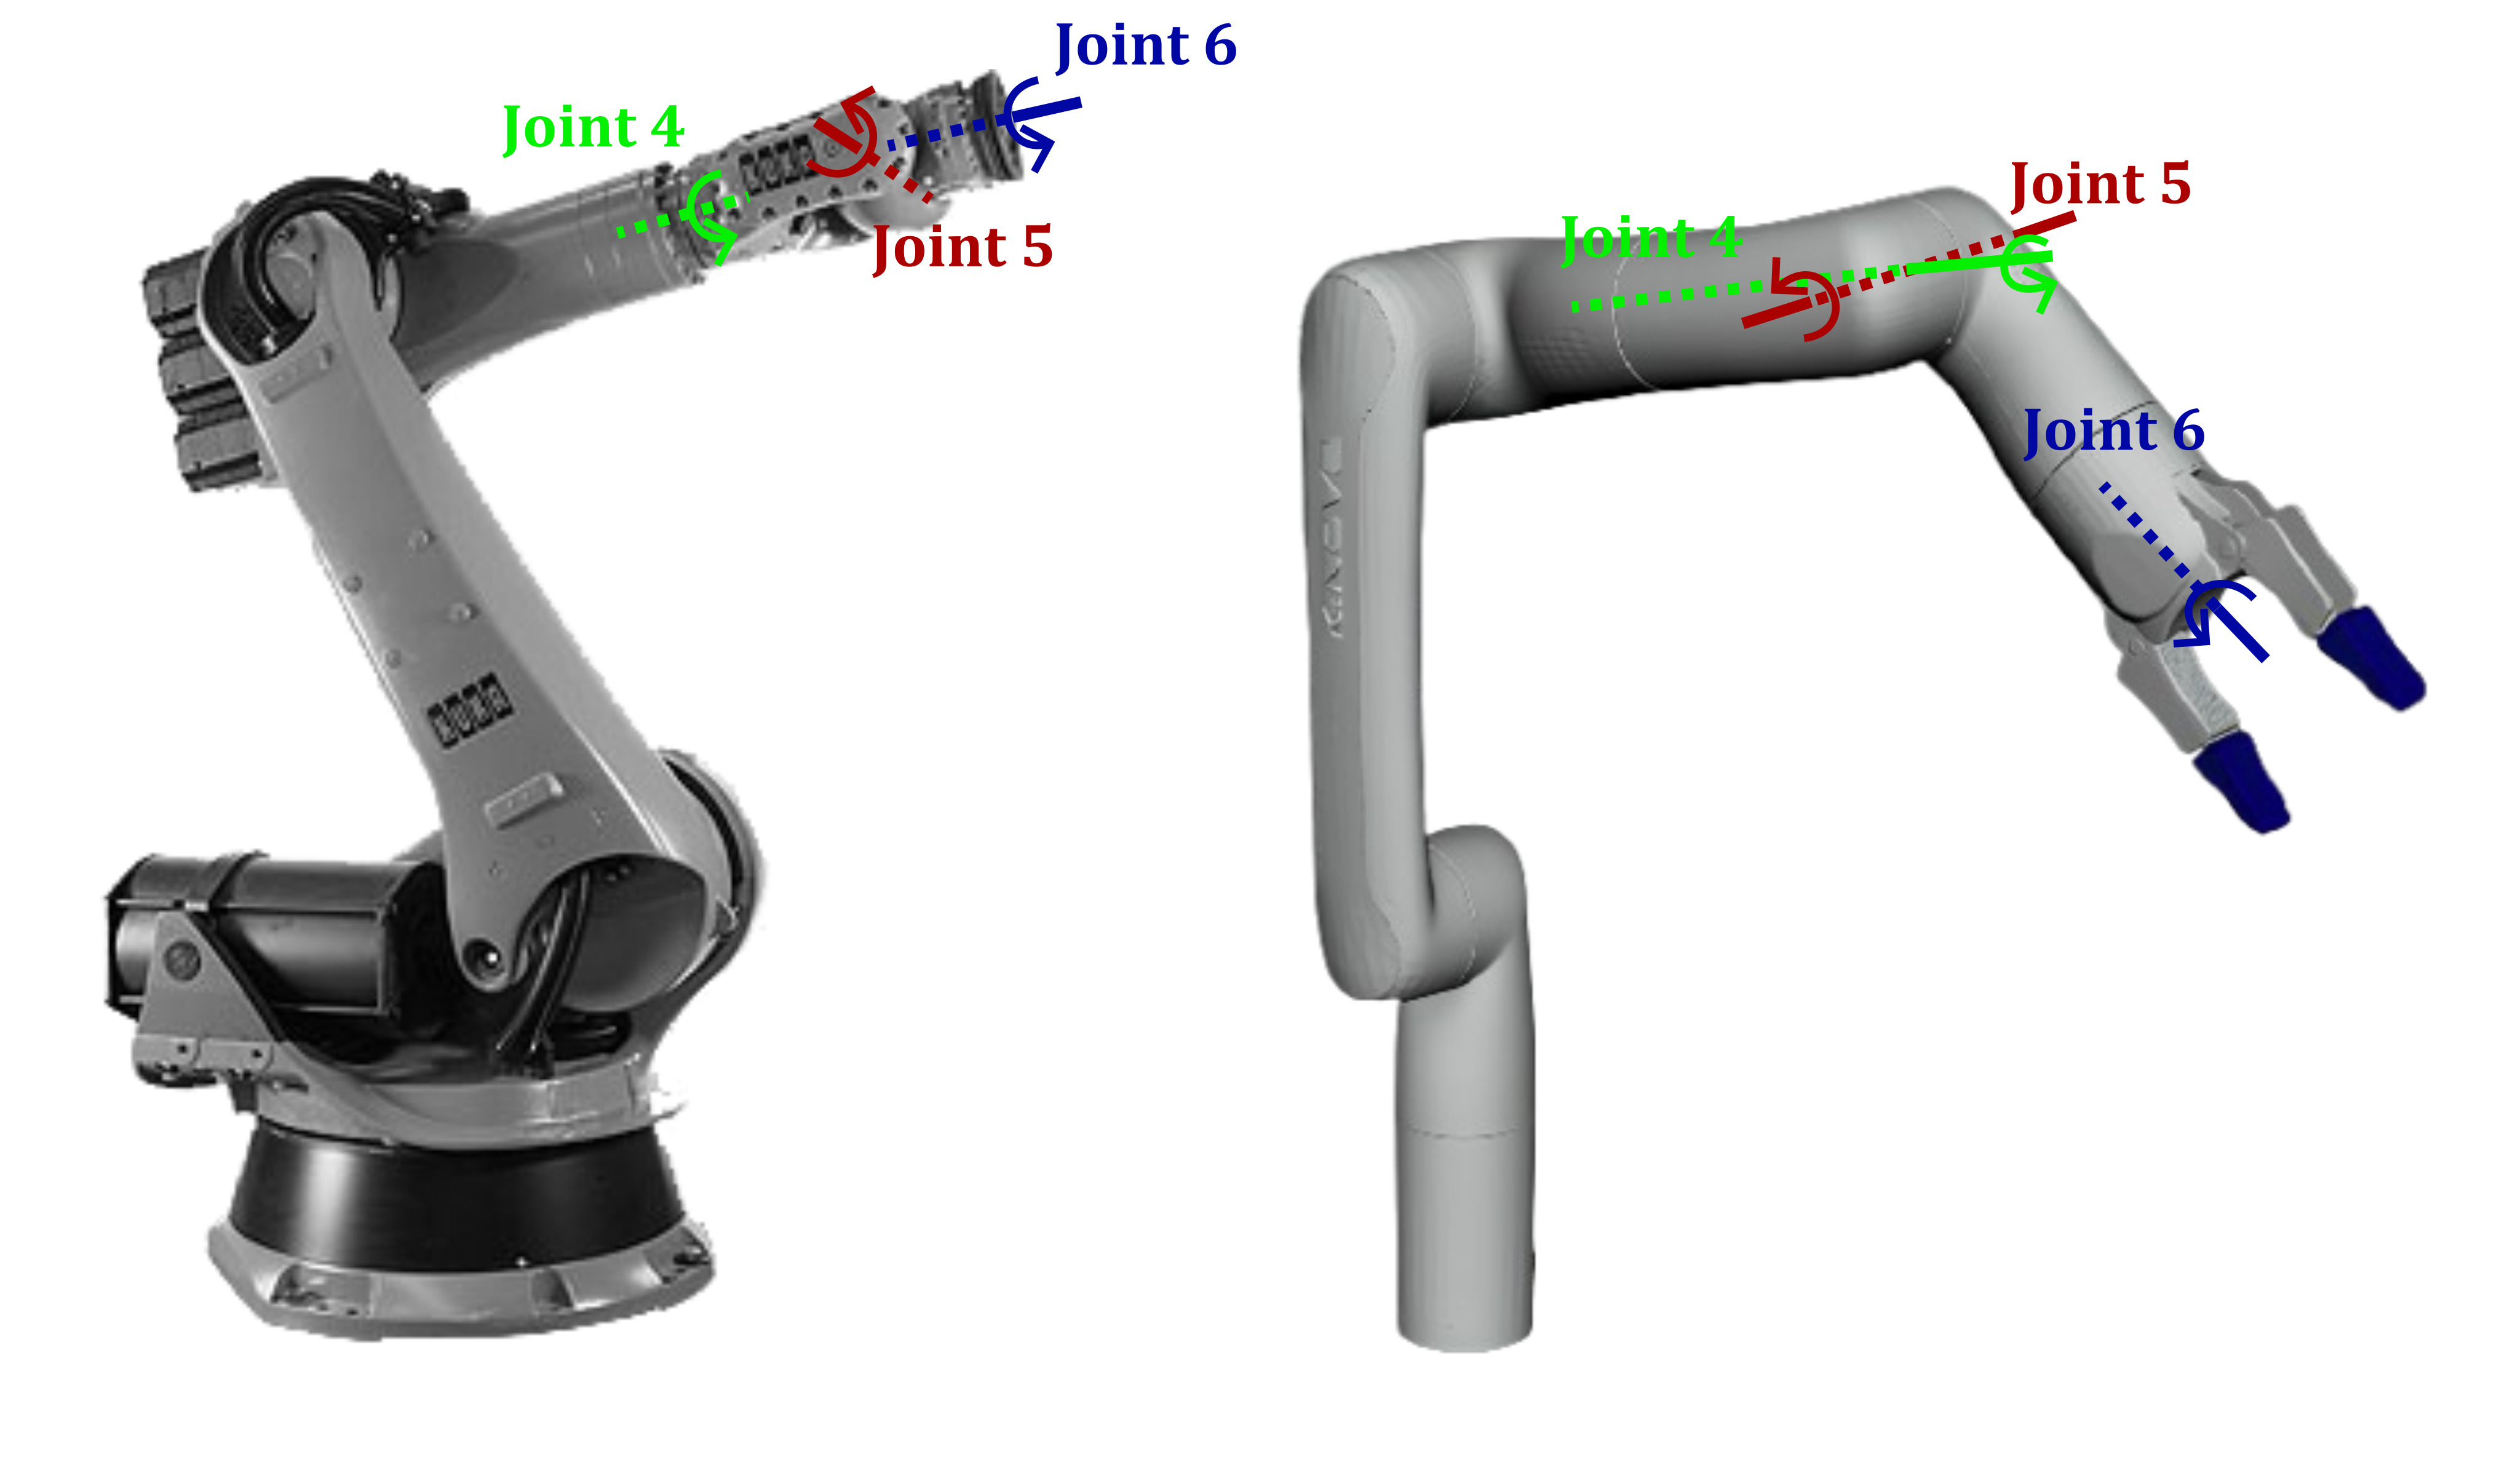
\includegraphics[width=\linewidth]{Fig_1.jpg}
    \caption{(a) KUKA KR-240 Manipulator with Spherical Wrist (b) Kinova Gen3 Lite Manipulator with Non-spherical Wrist}
    \label{fig:sphericalvsnonspherical}
\end{figure}

Modern industrial practices require far beyond standard pick and place operations \cite{intro_4}. Tasks such as continuous inspection and dynamic human-robot collaborative handoff increasingly require manipulators to track end-effector trajectories whose target poses are determined online and cannot be fully enumerated or precomputed in advance, in contrast to fixed, repeated motion profiles for which offline trajectory planning remains both sufficient and preferable \cite{11358968}. These operations require the manipulator to maintain a precise end-effector pose along a continuous Cartesian path, requiring joint velocity resolution at the hardware's closed-loop control frequency \cite{intro_6, intro_7}. However, for non-spherical wrist manipulators, this requirement introduces a fundamental kinematic bottleneck. The offset joint structure creates a unified, non-linear system where position and orientation are deeply coupled, requiring the inverse kinematics to be solved as a single optimization at every control timestep.

In this work, we present an end-to-end PPO-based differential inverse kinematics controller that directly maps instantaneous Cartesian pose errors to joint velocity commands, bypassing any dependence on numerical solvers or explicit Jacobian computation. A novel coupled reward function combining a min-operator pose reward, asymmetric progress shaping, and exponential energy penalty enforces simultaneous position-orientation convergence while producing smooth, hardware-safe velocity commands. Sim-to-real transfer is validated on physical Kinova Gen3 Lite hardware at 20 Hz.

The remainder of this paper is organized as follows: Sec~\ref{related work} surveys existing works on numerical IK solvers, velocity-level controllers, and learning-based approaches. Sec~\ref{method} details the proposed methodology, including the simulation environment, reward function design, and ablation studies validating each reward component. Sec~\ref{results} presents quantitative and qualitative comparisons of the proposed method against classical and learning-based baselines on simulation and our method on real hardware. Finally, Sec~\ref{conclusion} summarizes the conclusions drawn from this work and outlines directions for future research. Our contributions are summarized as follows:
\begin{itemize}
\item We design a coupled reward architecture, combining min-operator
pose coupling, asymmetric progress shaping, and an exponential energy
penalty that resolves simultaneous position-orientation convergence
for the kinematic coupling inherent to non-spherical wrist manipulators,
without manual inter-objective weighting or staged training curricula.
This reward formulation, rather than the choice of underlying optimizer,
constitutes the core engineering contribution of this work.

\item We establish, through identical-reward comparisons against
alternative on-policy and off-policy algorithms (TRPO, SAC), that the
proposed reward architecture is responsible for the controller's
accuracy-smoothness trade-off, with the choice of Proximal Policy
Optimization (PPO) as the optimizing algorithm an empirically justified
design decision rather than the source of the result.

\item We demonstrate that a controller trained purely on static,
joint-limit-aware reachable-pose samples with no trajectory
supervision, dynamic model, or task-specific retraining generalizes
zero-shot to four continuous trajectory geometries (circle, square,
lemniscate, 3-D Lissajous) in both simulation and physical hardware,
offering a reactive, online alternative to precomputed offline IK
pipelines for applications where target poses cannot be fully enumerated
in advance.
\end{itemize}

\section{Related Work}
\label{related work}
To address the general inverse kinematics problem, several classical methods like numerical, analytical, combination of both and heuristic frameworks have been used in literature \cite{ABDORSIERRA2022100597}. Iterative solvers like TRAC-IK \cite{tracik} are widely used for their system-agnostic ability to handle joint limits and multiple constraints. However, even with a previous joint-state seed and the Distance parameter for solution selection, TRAC-IK remains fundamentally trajectory-unaware, each waypoint is resolved as an independent optimization with no inter-waypoint coupling, leading to configuration-branch switching and joint-space discontinuities during continuous trajectory tracking. Similarly, heuristic methods such as Forward And Backward Reaching IK (FABRIK) \cite{fabrik} introduced, while computationally efficient but limited to position reaching applications, lack the necessary temporal awareness. In addition, analytical closed form solution proposed in \cite{zohour2021kinova}, reduces the complex kinematics of the robot into a single 16th-degree polynomial to calculate all possible joint configurations for a given pose. Without strict nearest joint constraints, continuous sub-millisecond tracking causes the solver to jump between completely different joint configurations.

Velocity-level controllers address this by operating directly in the differential domain. Resolved-rate motion control (RRMC) \cite{whiteney1969resolved} computes joint velocities using the Jacobian pseudo-inverse $(\dot{\theta}=J^{\dagger}\cdot\dot{x})$. While damped least squares(DLS)\cite{DLS, chiaverini1994review} introduce a damping factor $\lambda$ to prevent velocity singularities $(\dot{\theta} = J^\top(JJ^\top + \lambda^2 I)^{-1}\dot{x})$. Quadratic velocity-level  programming formulations \cite{velocityqp} further impose joint limit constraints explicitly, offering safer hardware deployment \cite{velocityqp_2}. These methods require an explicit, accurate Jacobian at every timestep.

To improve upon the accuracy limitations of classical velocity controllers, hybrid approaches have emerged combining numerical methods with learned components \cite{wang2023two}. Learning based methods has been explored as a residual corrector atop numerical solvers \cite{jia2019finite,chen2019neural}, compensating for solver inaccuracies. An actor-critic RL approach was introduced as a correction signal in joint velocity space to the augmented PD controller for trajectory tracking on a 6-DOF industrial manipulator \cite{pane2016actor}. A gradient-free, model-free Bayesian Markov Chain Monte Carlo (MCMC) RL policy search utilized to circular trajectory control on 2-DOF manipulator in simulation to optimize the PD controller \cite{aghaei2022real}. A Soft Actor Critic(SAC)-based outer-loop stochastic reference correction policy learned directly from the 7-DOF Baxter manipulator. Their approach augments an existing vendor provided hardware controller with bounded corrective actions as an inheritance rather than learning from the environment \cite{pavlichenko2022real}. Further, \cite{zhang2019trajectory_1} apply distributed PPO with LSTM and GAE to trajectory tracking on a 3-DOF SCARA robot and mobile robot, using random reference state initialization and an exponential position-error reward.

Further, a compound controller combining a Sliding Mode Controller (SMC) with SAC-based RL augmented by Lyapunov stability constraints is proposed for the trajectory tracking of manipulators \cite{liu2022reinforcement, mao2025real}. While their method requires a complete dynamic model of the system, it demonstrates that model-based initialization significantly improves RL sample efficiency. A hybrid framework combining Twin Delayed Deep Deterministic Policy Gradient (TD3) with an RRT-generated reference trajectory is proposed \cite{ota}. In this integrated planning and RL system, the reward function directly penalizes deviations from the RRT-based reference, constraining the agent to refine the pre-computed joint-space path. Further, \cite{V2025104178} formulate a collaborative PPO variant for tracking and vibration suppression of a flexible-joint manipulator, reporting that PPO-based policies converge faster and more stably than actor-critic and policy-gradient baselines under hardware-in-the-loop validation, a finding consistent with the convergence and
smoothness advantages of clipped on-policy optimization observed in the present work. In a similar way, \cite{li2021general} proposed a traditional path planner-DRL framework, combining RRT* with the Tsallis actor-critic algorithm to find optimized-energy IK solutions for redundant manipulators. This approach treats IK as a pose-reaching problem, solved point-by-point using an ANN-based solver.

Several DDPG-based methods have been explored to enhance trajectory tracking, these often depend on simplified assumptions or known dynamics. \cite{majumder2024enhancing} proposed a sequential DDPG approach for n-link manipulators, utilizing dual actor-critic networks trained progressively from 2D to 3D space to accelerate convergence. Similarly, \cite{zhang2019trajectory} implemented a distributed DDPG framework with prioritized experience replay, where multiple synchronous workers explore diverse policies to update a shared global network. Furthermore, \cite{hazem2025reinforcement} introduced hybrid variants, such as LC-DDPG and TD3-ADX, that learn joint torque commands by embedding an explicitly derived Euler-Lagrange dynamic model within the simulation. While these methods demonstrate efficacy in simulation, they frequently operate in joint torque space requiring precise manipulator dynamics, and lack real-time hardware validation, leaving the sim-to-real gap unaddressed. Moreover, these frameworks often overlook orientation control and motion smoothness, which are critical for scaling to 6-DOF manipulators.

Despite these advances trajectory tracking, specifically on non-spherical wrist manipulators is unaddressed, IK solution introduces kinematic coupling that complicates both analytical solvers and standard RL reward formulations. Existing approaches either operate in torque space requiring explicit dynamic models, augment pre-existing classical controllers rather than learning from scratch. Furthermore, no prior work demonstrates that a policy trained purely on static pose reaching over a joint limit aware reachability dataset, without any trajectory supervision can generalize to continuous trajectory tracking at deployment. The proposed framework addresses this gap directly: a compact
256$\times$256 actor-critic architecture, trained end-to-end on this
coupled reward, learns a generalizable velocity-level mapping that
naturally extends to arbitrary trajectory tracking without requiring
trajectory demonstrations, dynamic models, or task-specific re-training. 

% \begin{itemize}
%      \item A novel reward function combining inverse-quadratic pose reward via a min-operator, asymmetric progress shaping, and energy penalty that jointly drives position and orientation convergence without reward exploitation specifically designed for the kinematic coupling inherent in non-spherical wrist configurations.
%      \item The policy is trained purely on joint limit aware 1.5M reachable workspace poses with no trajectory supervision, yet learns a velocity-level differential IK mapping that generalizes to continuous trajectory tracking (circle, square, lemniscate, 3-D Lissajous) at deployment.
%  \end{itemize}

 \section{Methodology}
\label{method}
The proposed framework, illustrated in Fig.~\ref{fig:overallmethodology}, describes our methodology for training the trajectory tracking task. The observation space \textbf{$s_{t}$} $\in$ $\mathbb{R}^{19}$ provides the essential information required for the update of the policy. The action space \textbf{$a_{t}$} $\in$ $\mathbb{R}^{6}$ consists of six joint velocities sampled from the policy $\pi_\theta(\cdot|\mathbf{s}_\text{t})$. The training environment, implemented in NVIDIA Isaac Lab, utilizes 4096 parallel environments to train actor-critic neural networks with a $256\times256$ architecture. Further this setup uses Proximal Policy Optimization (PPO) to give efficient joint velocities for the efficient trajectory tracking explained below in further sections.
\subsection{State and Action Space}
The policy operates on a 19-dimensional observation vector as detailed in Tab~\ref{tab:obs_action} and outputs 6-dimensional joint velocity commands $\boldsymbol{\dot{\theta_{p}}}$.
\begin{figure}
    \centering
    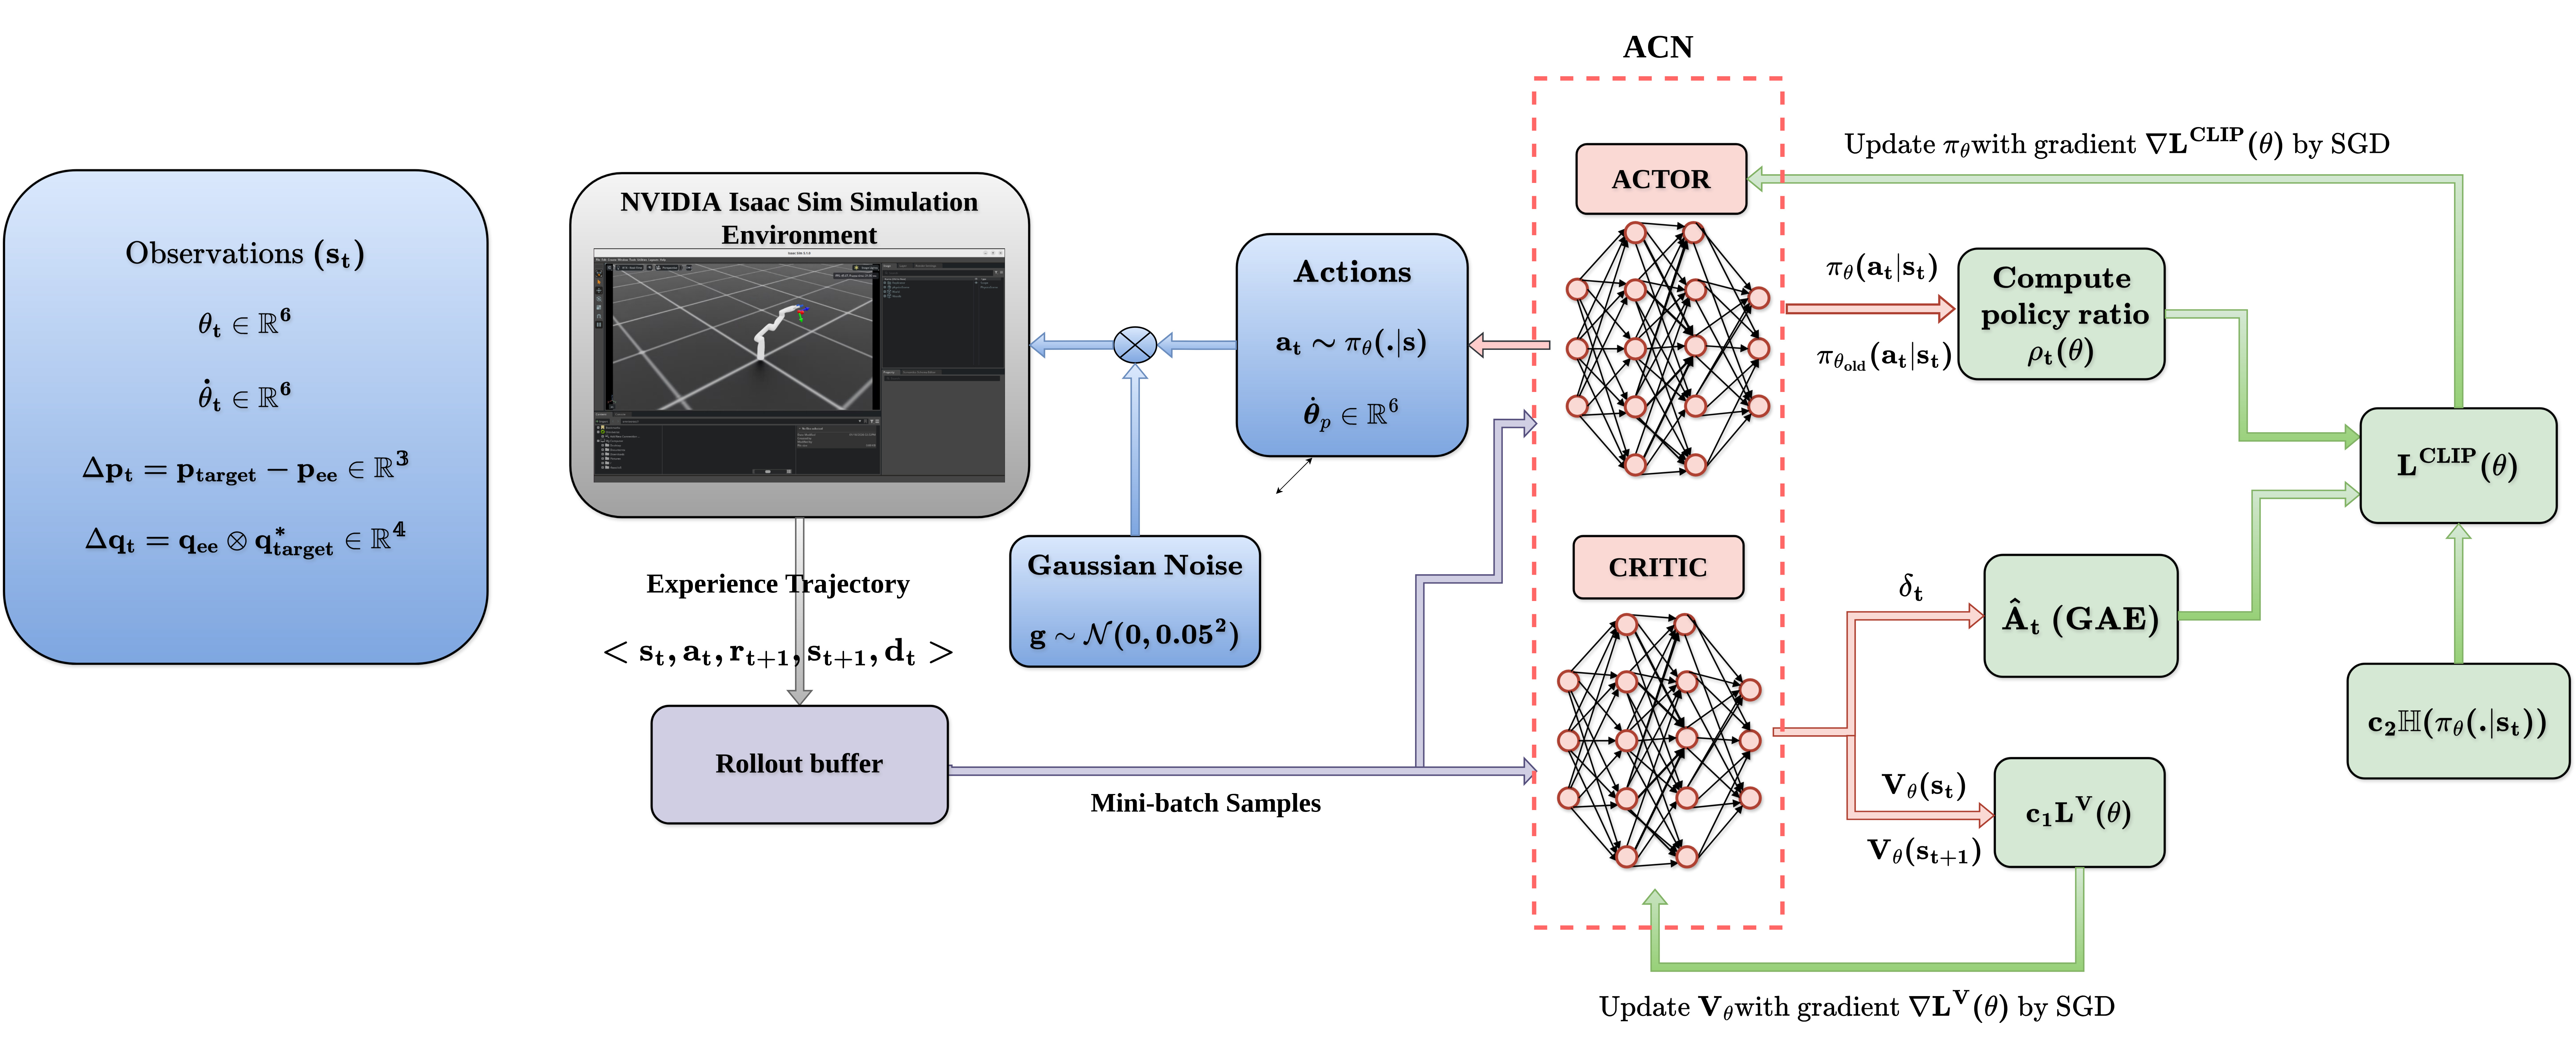
\includegraphics[width=\linewidth]{Fig_2_new.jpg}
    \caption{Overall Method for Differential Inverse Kinematics for Trajectory Tracking.}
    \label{fig:overallmethodology}
\end{figure}
\begin{table}[h]
\centering
\caption{Observation and Action Space}
\label{tab:obs_action}
\begin{tabular}{llcc}
\midrule
\textbf{Type} & \textbf{Description} & \textbf{Symbol} & \textbf{Dim.} \\
\midrule\midrule
\multirow{5}{*}{Observation} & Joint positions & $\boldsymbol{\theta}_t$ & 6 \\
                              & Joint velocities & $\dot{\boldsymbol{\theta}}_t$ & 6 \\
                              & Position error & $\Delta\mathbf{p}_t$ & 3 \\
                              & Orientation error & $\Delta\mathbf{q}_t$ & 4 \\
                              % &  Twist & $\mathit{V}_t$ & 6 \\
\midrule
Action & Joint velocity commands & $\dot{\boldsymbol{\theta}_{p}}$ & 6 \\
\midrule
\textbf{Total Observation} & & & \textbf{19} \\
\hline
\end{tabular}
\end{table}
\subsection{Simulation Environment}
\label{simulation}
Training is conducted in NVIDIA Isaac Lab with a physics timestep of $\Delta t$ = 1/120~s and a control decimation of 2, resulting in a policy frequency of 60Hz. The Kinova Gen3 Lite robot is modeled as a USD asset with self-collisions enabled, ensuring physically realistic interactions during training. The joints are velocity-controlled, enabling direct command of joint velocities from the policy output. Each episode spans 600~steps, with the robot initialized to its home configuration(zero position) at every reset. The set of reachable target poses used for episode initialization is
constructed offline via forward kinematics on the Kinova Gen3 Lite
kinematic model. Each of the six joints is swept independently across its
mechanical limit range at $5^{\circ}$ increments, and the full combinatorial
set of joint-angle tuples is mapped to the corresponding 6-DOF end-effector
pose. Candidate poses are filtered using Isaac Sim's contact-sensing
pipeline, discarding any joint configuration that produces self-collision,
retaining only collision-free, kinematically valid poses. This procedure
yields a fixed dataset of 1.5M reachable workspace poses, generated once
prior to training and reused unchanged across the full $5\times10^{8}$-step
training run. At every episode reset, a target pose is drawn uniformly at
random from this fixed set, and the corresponding pose error
($\Delta\mathbf{p}_t$, $\Delta\mathbf{q}_t$ in Table~\ref{tab:obs_action})
is computed relative to the robot's current end-effector pose. Stochasticity
during training is introduced not by perturbing the target pose set itself,
but at the policy output, via the additive Gaussian action noise of
Eq.~\ref{noise} (Sec~\ref{rollout}), which serves as the
domain-randomization mechanism discussed in Section~\ref{sim2real}. The training is conducted on an NVIDIA GeForce RTX 5060 Ti (16~GB VRAM) with the hyper parameters used are listed in Tab~\ref{tab:ppo_hyperparams}.

\begin{table}[h]
\centering
\caption{PPO Hyperparameters}
\label{tab:ppo_hyperparams}
\begin{tabular}{lc}
\midrule
\textbf{Hyperparameter} & \textbf{Value} \\
\midrule\midrule
Total Timesteps & $5\times 10^8$\\
Parallel Environments & 4096 \\
Steps per Rollout ($N_\text{steps}$) & 16 \\
Minibatch Size & 4096 \\
Number of Epochs & 10 \\
Discount Factor ($\gamma$) & 0.99 \\
GAE Parameter ($\lambda$) & 0.95 \\
Learning Rate & $5 \times 10^{-5}$\\
Clip Range ($\epsilon$) & 0.13 \\
Entropy Coefficient ($c_2$) & 0.01 \\
Value Function Coefficient ($c_1$) & 0.5 \\
Max Gradient Norm & 0.5 \\
Network Architecture & [$256 \times 256$]\\
Activation Function & Tanh \\
Weight Initialization & Orthogonal \\
\midrule
\end{tabular}
\end{table}

\subsection{Rollout Collection and Policy Update}
\label{rollout}
At each training iteration, experience tuples $\langle \mathbf{s}_\text{t}, \mathbf{a}_\text{t}, r_\text{t+1}, \mathbf{s}_\text{t+1}, \text{d}_{\text{t}} \rangle$ are collected across all parallel environments over $N_\text{steps}$ = 16 steps, yielding 65,536 transitions per rollout. The policy $\pi_\theta(\cdot|\mathbf{s}_\text{t})$ outputs a 6-dimensional joint velocity command $\dot{\boldsymbol{\theta}_{p}} \in \mathbb{R}^6$, one per actuated joint of the Kinova Gen3 Lite. To improve robustness to real hardware actuator imprecision and to encourage exploration of the joint velocity space, additive Gaussian perturbation noise, $g \sim \mathcal{N}(0, 0.05^2)$ is injected at the environment interface before command execution as in Eq.~\ref{noise}:  
\begin{equation}
\begin{split}
    \mathbf{a}_t &= \text{clip}\left(\pi_{\theta}(\cdot|\mathbf{s}_\text{t}) + g,\ -1,\ 1\right); \\ 
    & g \sim \mathcal{N}(0, 
    0.05^2\cdot\mathbf{I}_6)
\end{split}
\label{noise}
\end{equation}
This perturbation serves a dual purpose, prevents the policy from overfitting to the noiseless simulation dynamics and acts as implicit domain randomization, narrowing the sim-to-real gap at deployment. Advantage as in Eq.~\ref{advantage}, estimates are computed via Generalized Advantage Estimation(GAE) using the critic value $V_\theta(\mathbf{s}_t)$:
\begin{equation}
\begin{split}
    \hat{A}_\text{t} &= \sum_{l=0}^{N_\text{steps}} (\gamma\lambda)^l \delta_{t+l}; \\
    & \delta_\text{t} = r_\text{t} + \gamma V_\theta(\mathbf{s}_\text{t+1}) - V_\theta(\mathbf{s}_\text{t})
\end{split}
\label{advantage}
\end{equation}
with discount factor $\gamma = 0.99$ and GAE parameter $\lambda = 0.95$. The actor $\pi_\theta$
is updated by maximizing the objective as in Eq.~\ref{objective}:
\begin{equation}
L(\theta) = L^{\text{CLIP}}(\theta) - c_{1}\cdot L^{V}(\theta) + c_{2} \cdot\mathbb{H}(\pi_\theta(\cdot|\mathbf{s}_\text{t}))
\label{objective}
\end{equation}
where \[L^{\text{CLIP}}(\theta) = \mathbb{E}_\text{t}\left[\min\left(\rho_\text{t}(\theta)\hat{A}_\text{t},\ \text{clip}(\rho_\text{t}(\theta), 1 - \epsilon, 1 + \epsilon)\hat{A}_\text{t}\right)\right]\]
the policy ratio $\rho_\text{t}(\theta) = \pi_{\theta}(a_\text{t}|s_\text{t})/\pi_{\theta_{old}}(a_\text{t}|s_\text{t})$ measures the deviation from the previous policy, the clipping range $\epsilon$ is 0.13, constrains the update step. The critic is updated by minimizing
mean squared error between the predicted value and the target return $
L^{V}(\theta) = \mathbb{E}_\text{t}[(V_{\theta}(s_\text{t}) - \hat{R_\text{t}})^{2}]
$, and $\hat{R}_{t} = \hat{A}_{t} + V_{\theta}(s_{t})$ is the target return, value function coefficient $c_{1} = 0.5$, and entropy coefficient $c_{2}$ is 0.01. Both actor-critic networks are parameterized with Tanh activations and orthogonal initialization, updated jointly over 10 epochs per rollout via minibatch SGD with batch size 4096 as listed in Tab~\ref{tab:ppo_hyperparams}.
\subsection{Reward Shaping}
\label{reward_function}
Designing a reward function for trajectory tracking on non-spherical wrist manipulators requires careful balance between position and orientation error convergence. The proposed reward function simultaneously minimizes both, while enforcing progressive convergence and smooth joint motion. The proposed reward function consists of three main components.

\noindent \textbf{Pose Reward:}
The position and orientation errors are first normalized to a common scale:
\begin{equation}
    \begin{split}
    {\mathbf{\text{e}}}_{\text{p}} &= \frac{\|\mathbf{\text{p}}_\text{target} - \mathbf{\text{p}}_\text{ee}\|_{2}}{\text{d}_\text{max}}, \\ {\text{e}}_{\text{o}} &= \frac{2\cdot cos^{-1}(|\text{Re}(\mathbf{\text{q}}_\text{ee} \otimes \mathbf{\text{q}}_\text{target}^{*})|)}{\pi}
    \end{split}
    \label{pose_errors}
\end{equation}
where $\text{d}_{\text{max}}$ is the diagonal of the workspace, normalizing both errors ensures that the position and orientation errors are comparable in magnitude, preventing one from dominating the other.
The errors $\in\mathbb{R}$ as in Eq.~\ref{pose_errors}, then shaped through a combined inverse-quadratic and logarithmic term as in Eq.~\ref{position_error_reward}:
\begin{equation}
    r({\mathbf{\text{x}}}) = \frac{2.5}{1 + 100 \cdot \mathbf{\text{x}^{\text{2}}}}  - 0.1\log(\mathbf{\text{x}} + 1e^{-8})
    \label{position_error_reward}
\end{equation}
where $\text{x}$ is $\text{e}_\text{p/o}$.

\noindent The inverse-quadratic and logarithmic nature of the reward function helps to provide strong attraction in near-goal situations, and maintain a non-zero gradient far from the goal, avoiding the problem of sparse rewards.
The two terms are then coupled via a minimum operator as in Eq.~\ref{final_pose_reward}:
\begin{equation}
    r_\text{pose} = \min(r({\mathbf{\text{e}}}_\text{p}),\ r({\mathbf{\text{e}}}_\text{o}))
    \label{final_pose_reward}
\end{equation}
The unconstrained algebraic combination of position and orientation rewards is susceptible to reward exploitation, where the agent converges to a suboptimal policy by maximizing one objective while leaving the other unconstrained. The pose reward as shown in Eq.~\ref{final_pose_reward} applies, "\texttt{min}" operator to maintain simultaneous competency in both position and orientation throughout training. 

\noindent \textbf{Progress Reward:}
 Although the coupled pose reward shapes the magnitude of errors, it does not give an explicit incentive for the policy to reduce errors at every timestep. A policy could sustain a moderate error indefinitely and still receive a non-trivial reward. To address this, we introduce a progress reward as in Eq.~\ref{progress_reward}, that explicitly penalizes stagnation and rewards per-step error reduction.
 At each timestep, the per-step error delta $\in\mathbb{R}$ as in Eq.~\ref{change_in_error}, is computed for both position and orientation:
 \begin{equation}
    \Delta{\mathbf{\text{e}}}_\text{p} = {\mathbf{\text{e}}}_\text{p,t} - {\mathbf{\text{e}}}_\text{p,t-1}, \quad \Delta{\mathbf{\text{e}}}_\text{o} = {\mathbf{\text{e}}}_\text{o,t} - {\mathbf{\text{e}}}_\text{o,t-1}
    \label{change_in_error}
\end{equation}
where a negative delta indicates an improvement. Rather than applying progress rewards to both dimensions simultaneously, we apply it only to the dominant error, the dimension that is less in progress using the condition as in Eq.~\ref{progress_cond}:
\begin{equation}
    \Delta{\mathbf{\text{e}}} = \begin{cases} \Delta{\mathbf{\text{e}}}_\text{p} & \text{if } \Delta{\mathbf{\text{e}}}_\text{p} \geq \Delta{\mathbf{\text{e}}}_\text{o}\\ 
    \Delta{\mathbf{\text{e}}}_\text{o} & \text{if } \Delta{\mathbf{\text{e}}}_\text{p} < \Delta{\mathbf{\text{e}}}_\text{o}
    \end{cases}
    \label{progress_cond}
\end{equation}
The progress reward is then shaped asymmetrically to ensure a continuous gradient through zero:
\begin{equation}
    r_\text{prog}(\Delta{\mathbf{\text{e}}}) = \begin{cases} 4(-\Delta{\mathbf{\text{e}}} + 0.25)^{0.5} - 2 & \Delta{\mathbf{\text{e}}} < 0 
    \\ -2\exp(2\,\Delta{\mathbf{\text{e}}}) + 2 & \Delta{\mathbf{\text{e}}} \geq 0
    \end{cases}
    \label{progress_reward}
\end{equation}
\noindent by offsetting the equations in Eq.~\ref{progress_reward}, we prevent discontinuous reward cliffs that destabilize the value estimation. Square-root shaping on improvement provides diminishing returns for large progress steps, retarding aggressive overshooting. In contrast, the exponential penalty for regression imposes a sharply increasing penalty for error growth, creating a strong pressure on monotonic convergence.

\noindent \textbf{Energy Penalty:}
Trajectory tracking demands not only accurate end-effector pose reaching, but also smooth, continuous joint movements throughout the trajectory tracking. To enforce smooth motion throughout the entire trajectory, we introduce a continuous energy penalty on joint velocity commands at every timestep as in Eq.~\ref{energy_penalty}:
\begin{equation}
r_\text{energy} = 1 - \exp\left(0.2\sum_{i=1}^{6}\dot{\boldsymbol{\theta}}_i^2\right)
\label{energy_penalty}
\end{equation}
the exponential formulation imposes a sharply increasing cost as the aggregate joint velocity increases.

\noindent The total reward is summation of pose, progression, and energy components as in Eq.~\ref{total_sum}.
\begin{equation}
r_\text{t+1} = r_\text{pose} + r_\text{prog} + r_\text{energy}
\label{total_sum}
\end{equation}
\subsection{Sim-to-Real Transfer}
\label{sim2real}
Deploying the trained policy on physical hardware requires bridging the gap between simulation dynamics and real actuator behavior(see Fig.~\ref{fig:sim2real}). At deployment, the policy output is clipped to $[-1, 1]$ before transmission to the Kinova Kortex API as in Eq.~\ref{hardware_joint_velocity}:
\begin{equation}
\dot{\boldsymbol{\theta}}_\text{p} = \text{clip}(\mathbf{a}_t, -1, 1) \cdot \frac{180}{\pi} \quad {\circ/s}
\label{hardware_joint_velocity}
\end{equation}
\begin{figure}
    \centering
    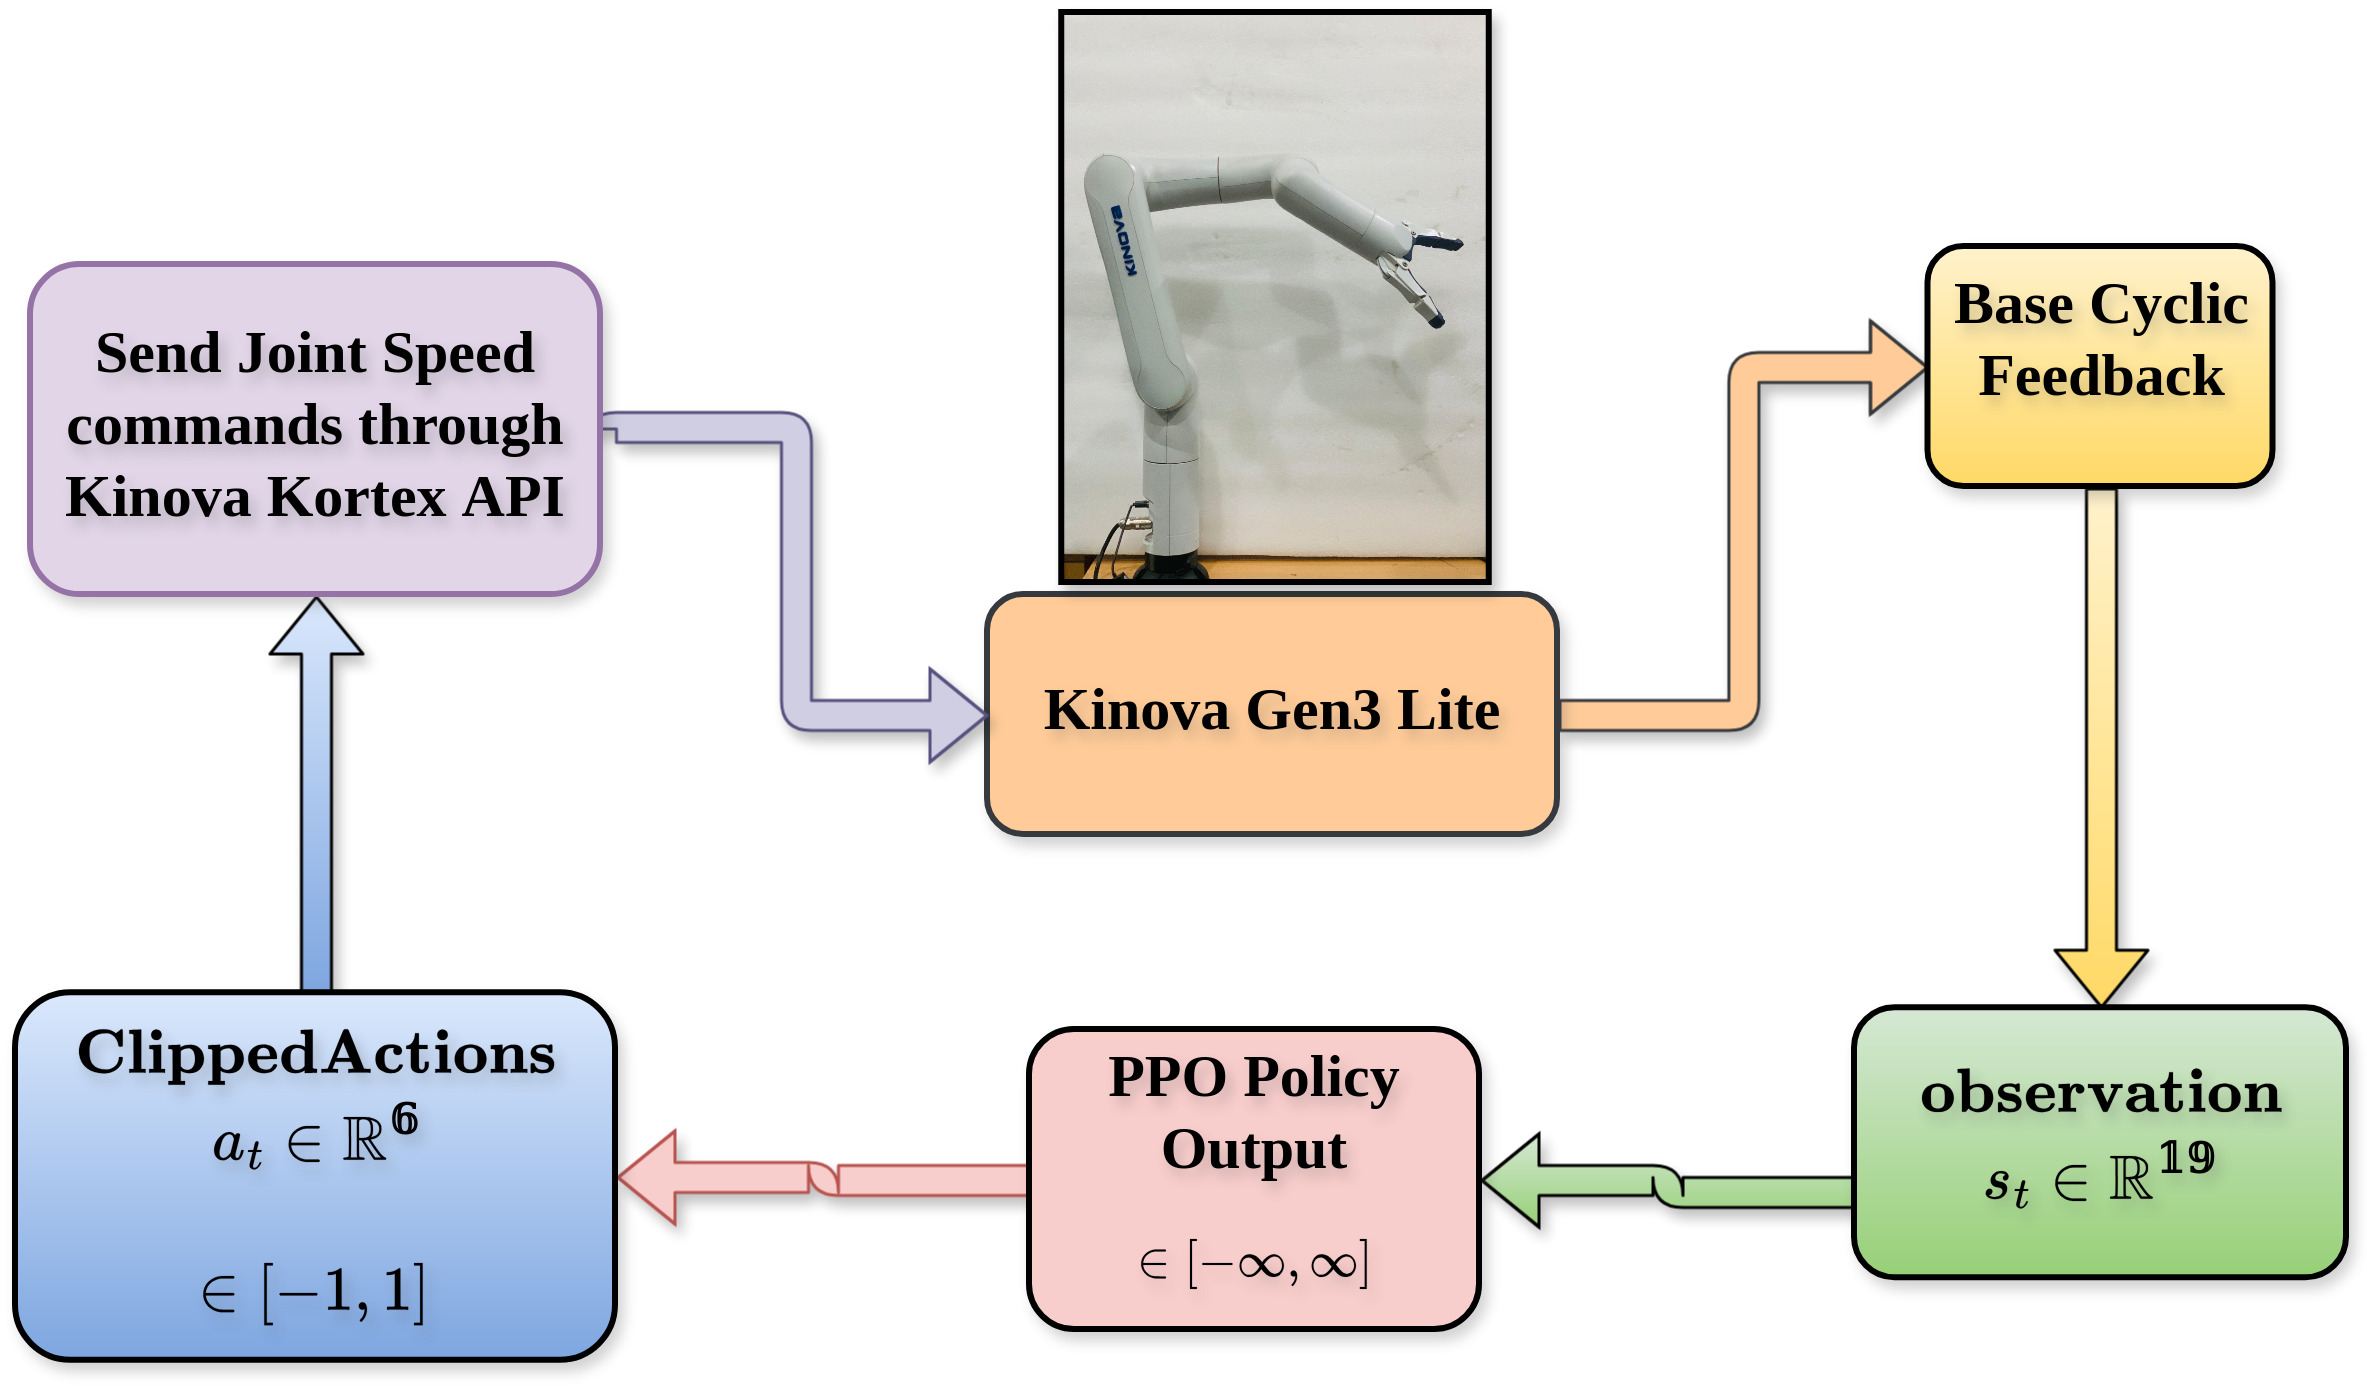
\includegraphics[width=\linewidth]{Fig_3_new.jpg}
    \caption{Sim-to-Real Architecture}
    \label{fig:sim2real}
\end{figure}
\noindent converting from normalized radians to degrees per second as required by the hardware interface. Observation parity between simulation and hardware is maintained directly from actuator feedback through the Kinova Kortex API, preserving the exact observation structure $\mathbf{s}_\text{t} \in \mathbb{R}^{19}$ seen during training. 

The policy is deployed on an Intel NUC9 Extreme (16-core CPU, 32~GB RAM), achieving inference at $\approx$1.3~kHz. The Kinova Gen3 Lite operates with a feedback and command frequency of $\approx$40~Hz each, imposed by the Kinova Kortex API. Since feedback reading and joint speed command dispatch are executed sequentially, the effective closed-loop control frequency is 20~Hz, well within real-time control requirements.

This 20~Hz effective control frequency is approximately one-third of the
60~Hz frequency used during training. Since the policy is a memoryless
mapping from instantaneous observation to velocity command with no
recurrent state, a lower deployment frequency only extends the
zero-order-hold (ZOH) duration of each command, it does not invalidate
any individual policy input. The per-step Gaussian action noise (Eq.~\ref{noise}) and energy penalty (Eq.~\ref{energy_penalty}) used during training jointly bound output velocity magnitude, limiting the inter-sample integration error introduced by a longer hold. Consistent with this, no frequency-related degradation was observed: hardware position RMSE on the circular trajectory (6.3~mm) was lower than simulation RMSE (9.95~mm) at the tested trajectory speed ($0.1$~rad/s), likely aided by actuator damping and the low-level joint velocity controller smoothing the discretized commands. This should be read as evidence against degradation at the tested speed, not as general frequency invariance; robustness at substantially higher tracking speeds, where pose error drifts more within a single 50~ms interval, remains untested and is left to future work.

Joint velocity commands are bounded by hardware velocity limits enforced at the actuator level and further soft-constrained by the exponential energy penalty in Eq.~\ref{energy_penalty}, which imposes a sharply increasing cost on aggregate joint speed. The hard clipping of policy outputs to $[-1,1]$ before dispatch provides an additional safety bound at both the simulation and hardware interfaces. Joint position limits are implicitly respected through Isaac Lab's physics solver.

\subsection{Baseline Comparison for Trajectory Tracking}
\label{reward_ablation}
To learn smooth and stable trajectory tracking, we rigorously evaluated existing DRL methods. Fig.~\ref{fig:training_curves} illustrates their mean terminal reward progression through training steps, normalized with respective maximum possible values to ensure fair comparison between differing reward structures.

The performance divergence between PPO and SAC highlights a critical trade-off between gradient stability and sample efficiency in trajectory tracking. While SAC is widely regarded as a strong baseline for continuous control, our results demonstrate that for confined-motion trajectory tracking, PPO's on-policy clipping mechanism provides a superior inductive bias. By constraining the probability ratio between successive policy updates, PPO suppresses high-frequency velocity fluctuations and actuator chattering that afflict off-policy methods under complex dense reward formulations. This is evident in Fig.~\ref{fig:training_curves}, PPO-D achieves monotonic improvement, effectively filtering the conflicting gradients introduced by energy penalties and progression rewards, converging to a smooth control law with a mean terminal reward of $\approx$ 0.93. Conversely, SAC-D substantially underperforms its sparse counterpart (SAC-S), indicating a failure in Q-value credit assignment. SAC's maximum entropy objective encourages exploratory joint movements that directly conflict with the energy penalty, causing the agent to settle into an idle local optimum that minimizes metabolic cost at the expense of task progress. 

TRPO-D, despite sharing PPO's conservative update logic through an exact KL-divergence constraint, converges slower and plateaus at a notably lower terminal reward $\approx$ 0.71, suggesting that the computational overhead of enforcing tight trust region boundaries impedes timely policy refinement compared to PPO's more tractable clipping approximation under dense reward supervision. PPO-S's stagnation at $\approx$0.12 reveals that without dense reward shaping, the agent receives feedback too infrequently to learn the precise joint coordination required for long-horizon differential IK trajectories. The sparse signal simply cannot distinguish between partially correct and fully correct motion sequences. Together, these results suggest that neither reward structure nor algorithm choice alone determines performance rather, it is their interaction dense rewards are necessary for precise credit assignment, but only on-policy optimization is robust to the conflicting gradients they introduce. For reactive trajectory tracking applications where target poses are determined online rather than precomputed, path fidelity and steady-state precision are paramount, and PPO-D's stable, variance-controlled optimization proves more technically suited to this requirement than the alternative on-policy and off-policy baselines evaluated here.

Wall-clock training cost varies substantially across methods
(Table~\ref{tab:wallclock}). TRPO-D requires 3h 14m 36s to complete
training, roughly $3\times$ PPO-D's 1h 5m 35s, consistent with the
overhead of its exact KL-divergence constraint discussed above. SAC-D
was trained for approximately $9\times10^{8}$ steps, nearly double
SAC-S's $4\times10^{8}$ step run, in the expectation that the dense
reward would eventually outperform its sparse counterpart given
sufficient additional experience; despite this extended budget, SAC-D's
terminal reward (Fig.~\ref{fig:training_curves}) remains well below
SAC-S's, reinforcing rather than resolving the entropy-energy conflict
discussed above, and its 2h 52m 34s wall-clock cost reflects this longer
run rather than a higher per-step cost. PPO-S terminates fastest
(38m 52s) due to early stagnation detection. These figures should be
read alongside \cite{zohour2021kinova}'s zero-cost closed-form analytical
solution for the same arm: the proposed method's accuracy and robustness
gains come at a one-time, sub-2-hour training cost, not a per-deployment
cost, and the policy requires no retraining across the four evaluated
trajectory geometries.
\begin{figure}
    \centering
    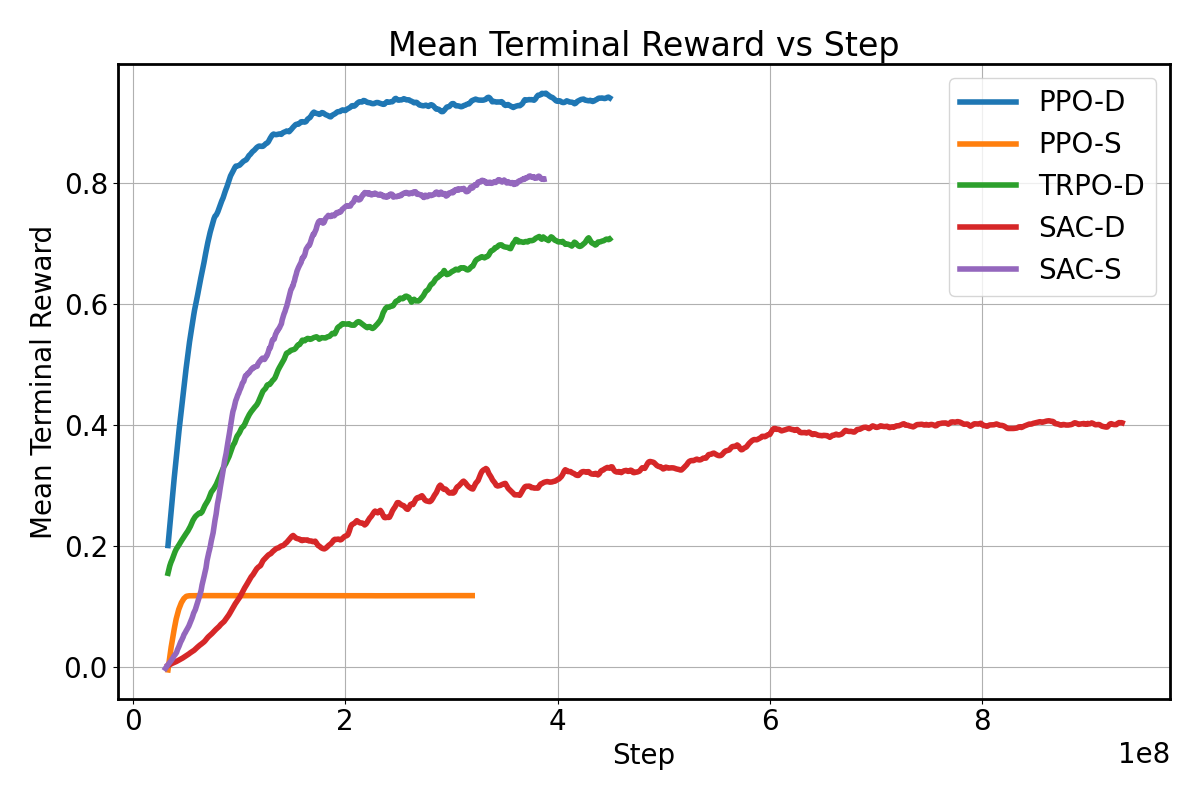
\includegraphics[width=0.8\linewidth]{Fig_4.png}
    \caption{Training Curves for PPO Dense Reward, PPO Sparse Reward, TRPO Dense Reward, SAC Dense Reward, and SAC Sparse Reward}
    \label{fig:training_curves}
\end{figure}
\begin{table}[h]
\centering
\caption{Wall-clock training time and total timesteps per algorithm.}
\label{tab:wallclock}
\begin{tabular}{lcc}
\hline
Method & Total Timesteps & Wall-clock time \\
\hline
PPO-D (proposed) & $\approx5\times10^{8}$ & 1h 05m 35s \\
PPO-S & $\approx3.5\times10^{8}$ & 38m 52s \\
TRPO-D & $\approx5\times10^{8}$ & 3h 14m 36s \\
SAC-D & $\approx9\times10^{8}$ & 2h 52m 34s \\
SAC-S & $\approx4\times10^{8}$ & 1h 24m 01s \\
\hline
\end{tabular}
\end{table}
\subsection{Reward Component Ablation Study}
The proposed reward function in Eq.~\ref{total_sum}, is validated to showcase the importance of each component in stable and smooth trajectory tracking. We evaluated four variants (a) Conventional, (b) Min Rew + Error Progression Reward, (c) Min Rew + Energy Penalty, and (d) Full reward. 
\begin{figure}
    \centering
    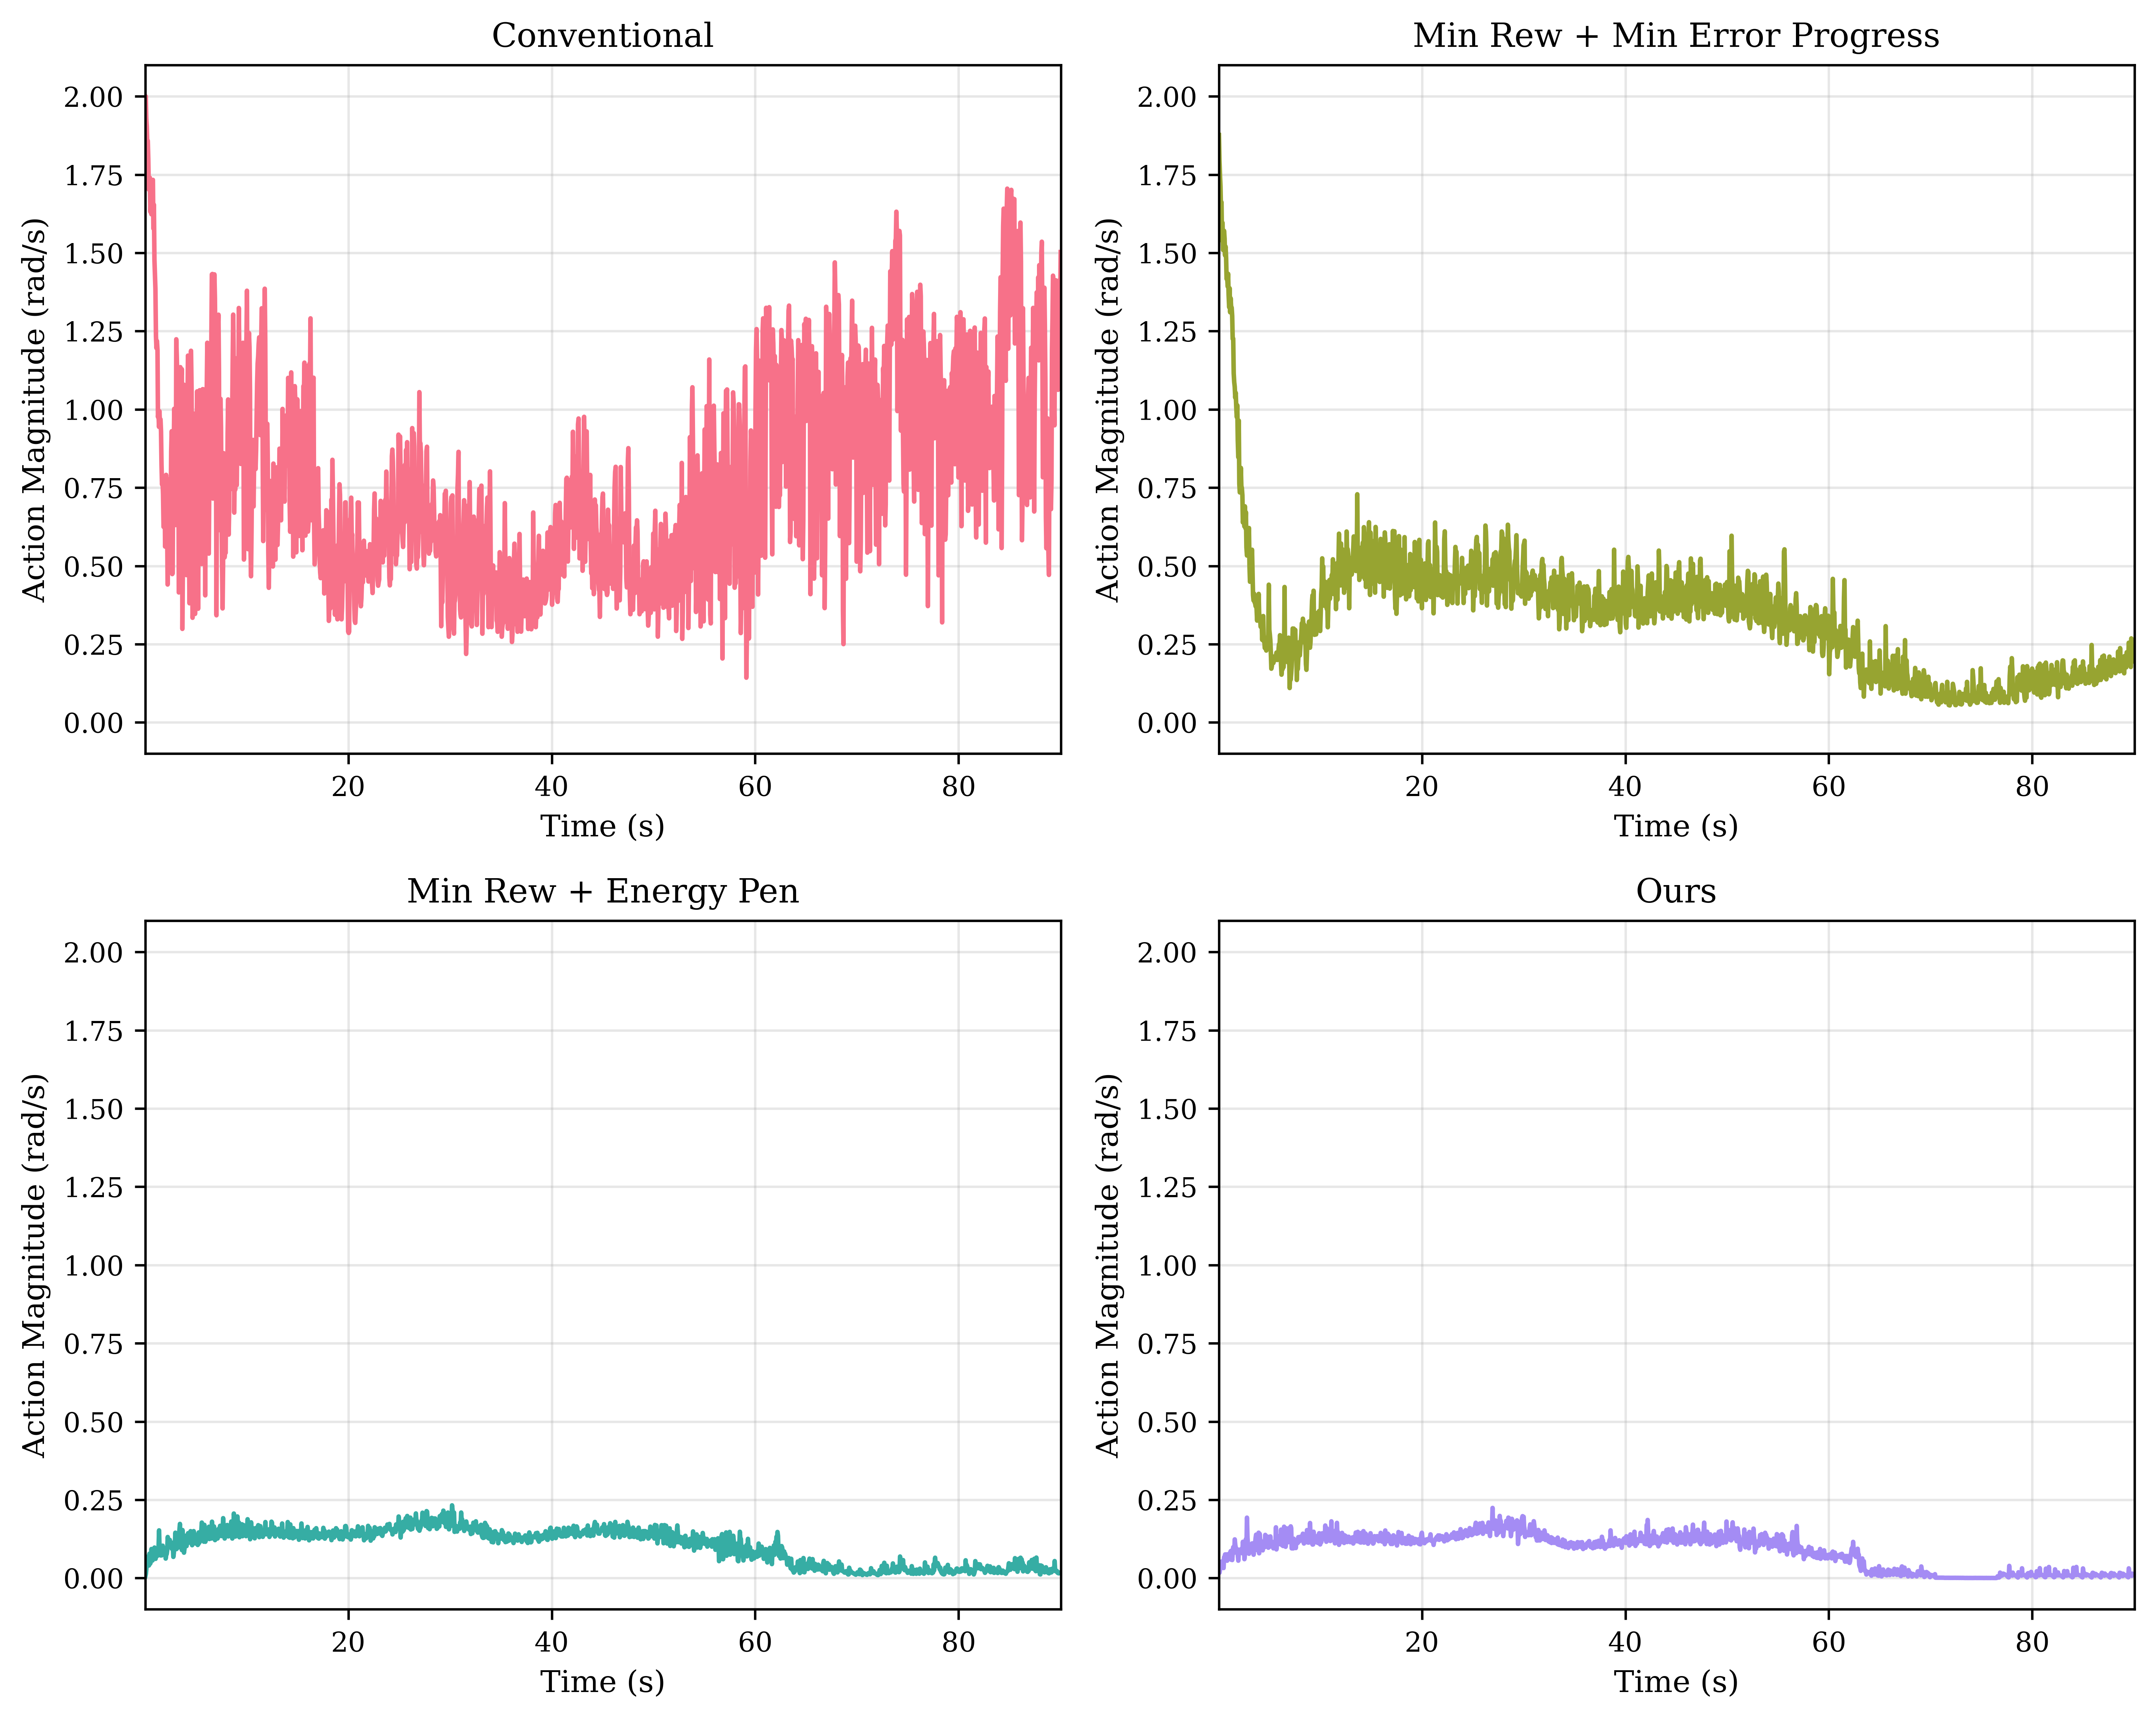
\includegraphics[width=\linewidth]{Fig_5.png}
    \caption{Joint Velocity Command Magnitudes across reward ablation variants
    during circular trajectory tracking: (a) Conventional, (b) Min Reward +
    Error Progression Reward, (c) Min Reward + Energy Penalty, (d) Full reward
    (ours). The exponential energy penalty in variants (c) and (d) suppresses
    peak action magnitude relative to (a) and (b).}
    \label{fig:action_magnitude}
\end{figure}
\begin{figure}
    \centering
    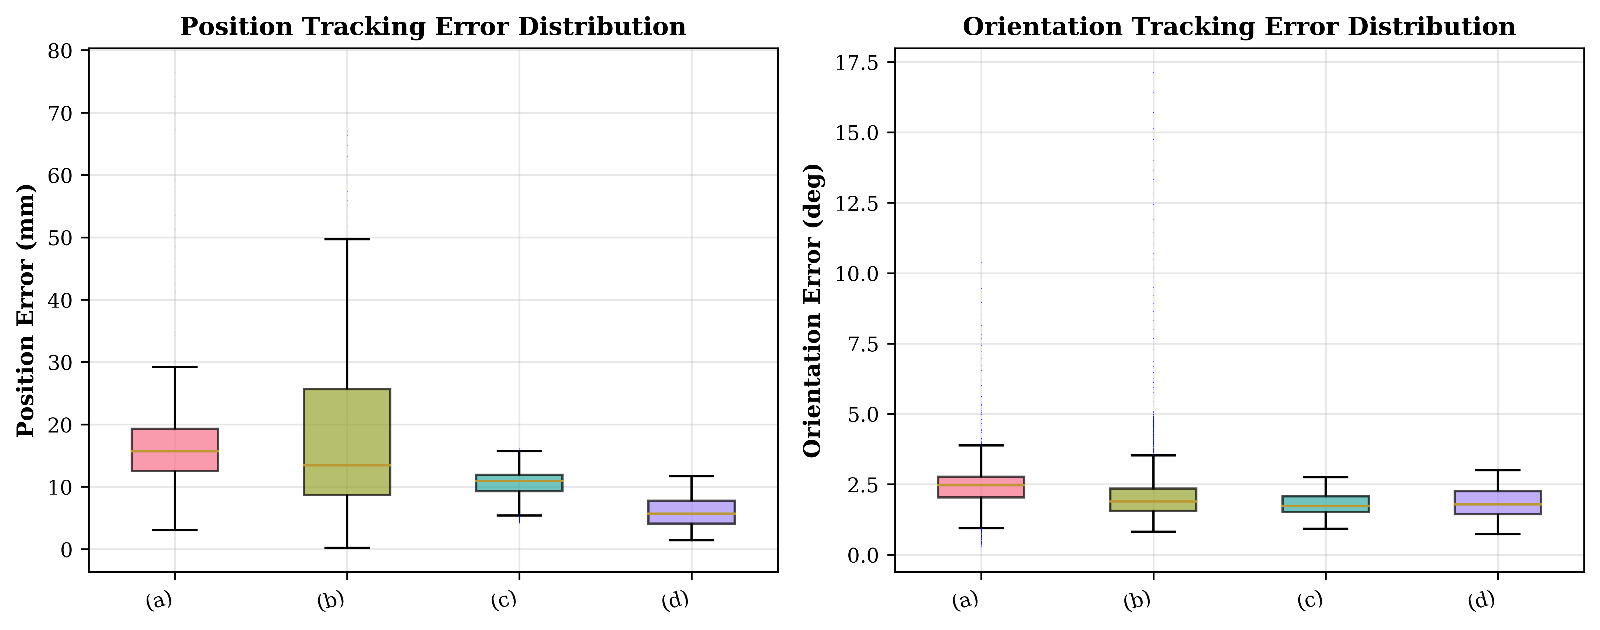
\includegraphics[width=\linewidth]{Fig_6.jpeg}
    \caption{Position and Orientation Tracking Error Distribution across
reward ablation variants on circular trajectory tracking. Variants (a)-(d)
as in Fig.~\ref{fig:action_magnitude}.}
    \label{fig:boxplots}
\end{figure}
For ablation studies, the circular trajectory considered across all the listed variants.

The exponential energy penalty directly suppresses joint velocity magnitude, reducing peak actions from 2.0~rad/s in the conventional reward to below 0.25 rad/s in our full reward as shown in Fig.~\ref{fig:action_magnitude}. The min-operator pose reward prevents the policy from exploiting high-velocity commands to satisfy one error dimension while neglecting the other. This coupling effect is visible in variant (b), where error progression without the energy penalty produces large transient velocity spikes before collapsing into erratic oscillations throughout the trajectory.

From Fig.~\ref{fig:boxplots}, the conventional reward(a) maintains persistent oscillations of 15–20~mm  throughout, never settling below the threshold. Variant (c) achieves stable sub-threshold tracking but with a higher steady-state median of ~10 mm. The full reward (d) achieves the lowest median position error of ~6 mm with the tightest distribution, consistently tracking below the 10 mm threshold across the entire trajectory, demonstrating that all three reward components are necessary for robust and smooth tracking. In addition, these four variants for tracking circular trajectory as shown in Fig.~\ref{fig:Circle_trajec}, the conventional reward (a) fails to complete the circular path, deviating significantly near the starting point. The Variant (b) completes the circle but with visible radial deviation. Variants (c) and (d) closely follow the desired trajectory, with (d) achieving near-perfect circular tracking.

\begin{figure}
    \centering
    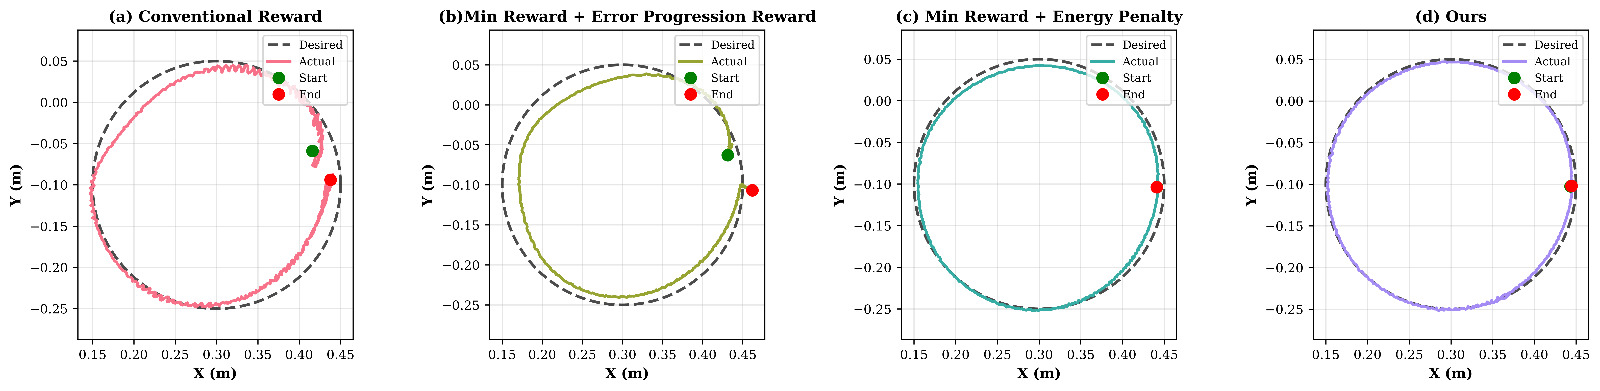
\includegraphics[width=\linewidth]{Fig_7.jpeg}
    \caption{XY Trajectory comparison across reward ablation variants on circular trajectory tracking. Variants (a)-(d) as in Fig.~\ref{fig:action_magnitude}.}
    \label{fig:Circle_trajec}
\end{figure}
\section{Results and Discussion}
\label{results}
% This section presents experimental validation on the Kinova Gen3 Lite in both simulation and physical hardware. The proposed method is evaluated on a circular trajectory against the baseline algorithms. All classical baselines were configured with parameters from their respective foundational works, DLS with $\lambda$ = 0.05, QP with minimum regularization ($\lambda$ = $10^{-3}$), and TRAC-IK seeded with the current joint state using the Distance optimization method, the configuration most favorable for inter-waypoint continuity. TRAC-IK, DLS, and SAC are additionally validated on physical hardware for the circular trajectory, while our method is further evaluated on lemniscate, 3-D Lissajous, and square trajectories. 
This section presents experimental validation on the Kinova Gen3 Lite in
both simulation and physical hardware. Sec~\ref{sim_result} compares the proposed method against five classical and learning-based baselines in simulation across three trajectory geometries, circle, lemniscate, and 3-D
Lissajous, chosen to span fixed-orientation, periodically-varying
orientation, and high-curvature multi-axis motion respectively. In Sec~\ref{real_time_deployment}, evaluated sim-to-hardware transfer on a physical Kinova Gen3 Lite, where TRAC-IK, DLS, and SAC, one representative baseline per method family, are additionally deployed on the circular trajectory, while the proposed method is further evaluated on 3-D Lemniscate, 3-D Lissajous, and square trajectories without retraining. All classical baselines retain the parameters reported in their respective foundational works, DLS with $\lambda = 0.05$ and QP with minimum regularization ($\lambda = 10^{-3}$); TRAC-IK is seeded with the current joint state using the Distance optimization method, the configuration most favorable for inter-waypoint continuity. Closed-loop configuration, per-method action scaling, and trajectory parameters common to both simulation and hardware trials are detailed in Sec~\ref{sim_result}.

\subsection{Simulation Result}
\label{sim_result}
All comparisons are carried out in the Nvidia Isaac Sim simulation
environment on circular, lemniscate, and 3-D Lissajous trajectories
(Tab~\ref{tab:error_metrics_sim}), with end-effector overlays shown for circle and 3-D Lissajous in Fig.~\ref{fig:plots_comparison} and Fig.~\ref{fig:plots_comparison_2}. All baselines and the proposed method operate under closed-loop Cartesian feedback: the velocity-level baselines (DLS, QP) recompute the Jacobian and pose error at every control timestep
rather than integrating open-loop, and TRAC-IK is re-seeded from the
current joint state at every waypoint. Per-method action scales as in Tab~\ref{tab:error_metrics_sim} were tuned on the circular trajectory to equalize each method's native output magnitude to the robot's velocity limits, then frozen and applied identically across all subsequent trajectories.

 % All comparisons are carried out in the Nvidia Isaac Sim simulation environment on circular and 3-D Lissajous trajectories. The end-effector trajectories against ground truth for all six methods, as shown in Fig.~\ref{fig:plots_comparison} and Fig.~\ref{fig:plots_comparison_2}, provide the capability of trajectory tracking of each method respectively, and the RMSE values listed in Tab~\ref{tab:error_metrics_sim}. 
\begin{figure}
    \centering
    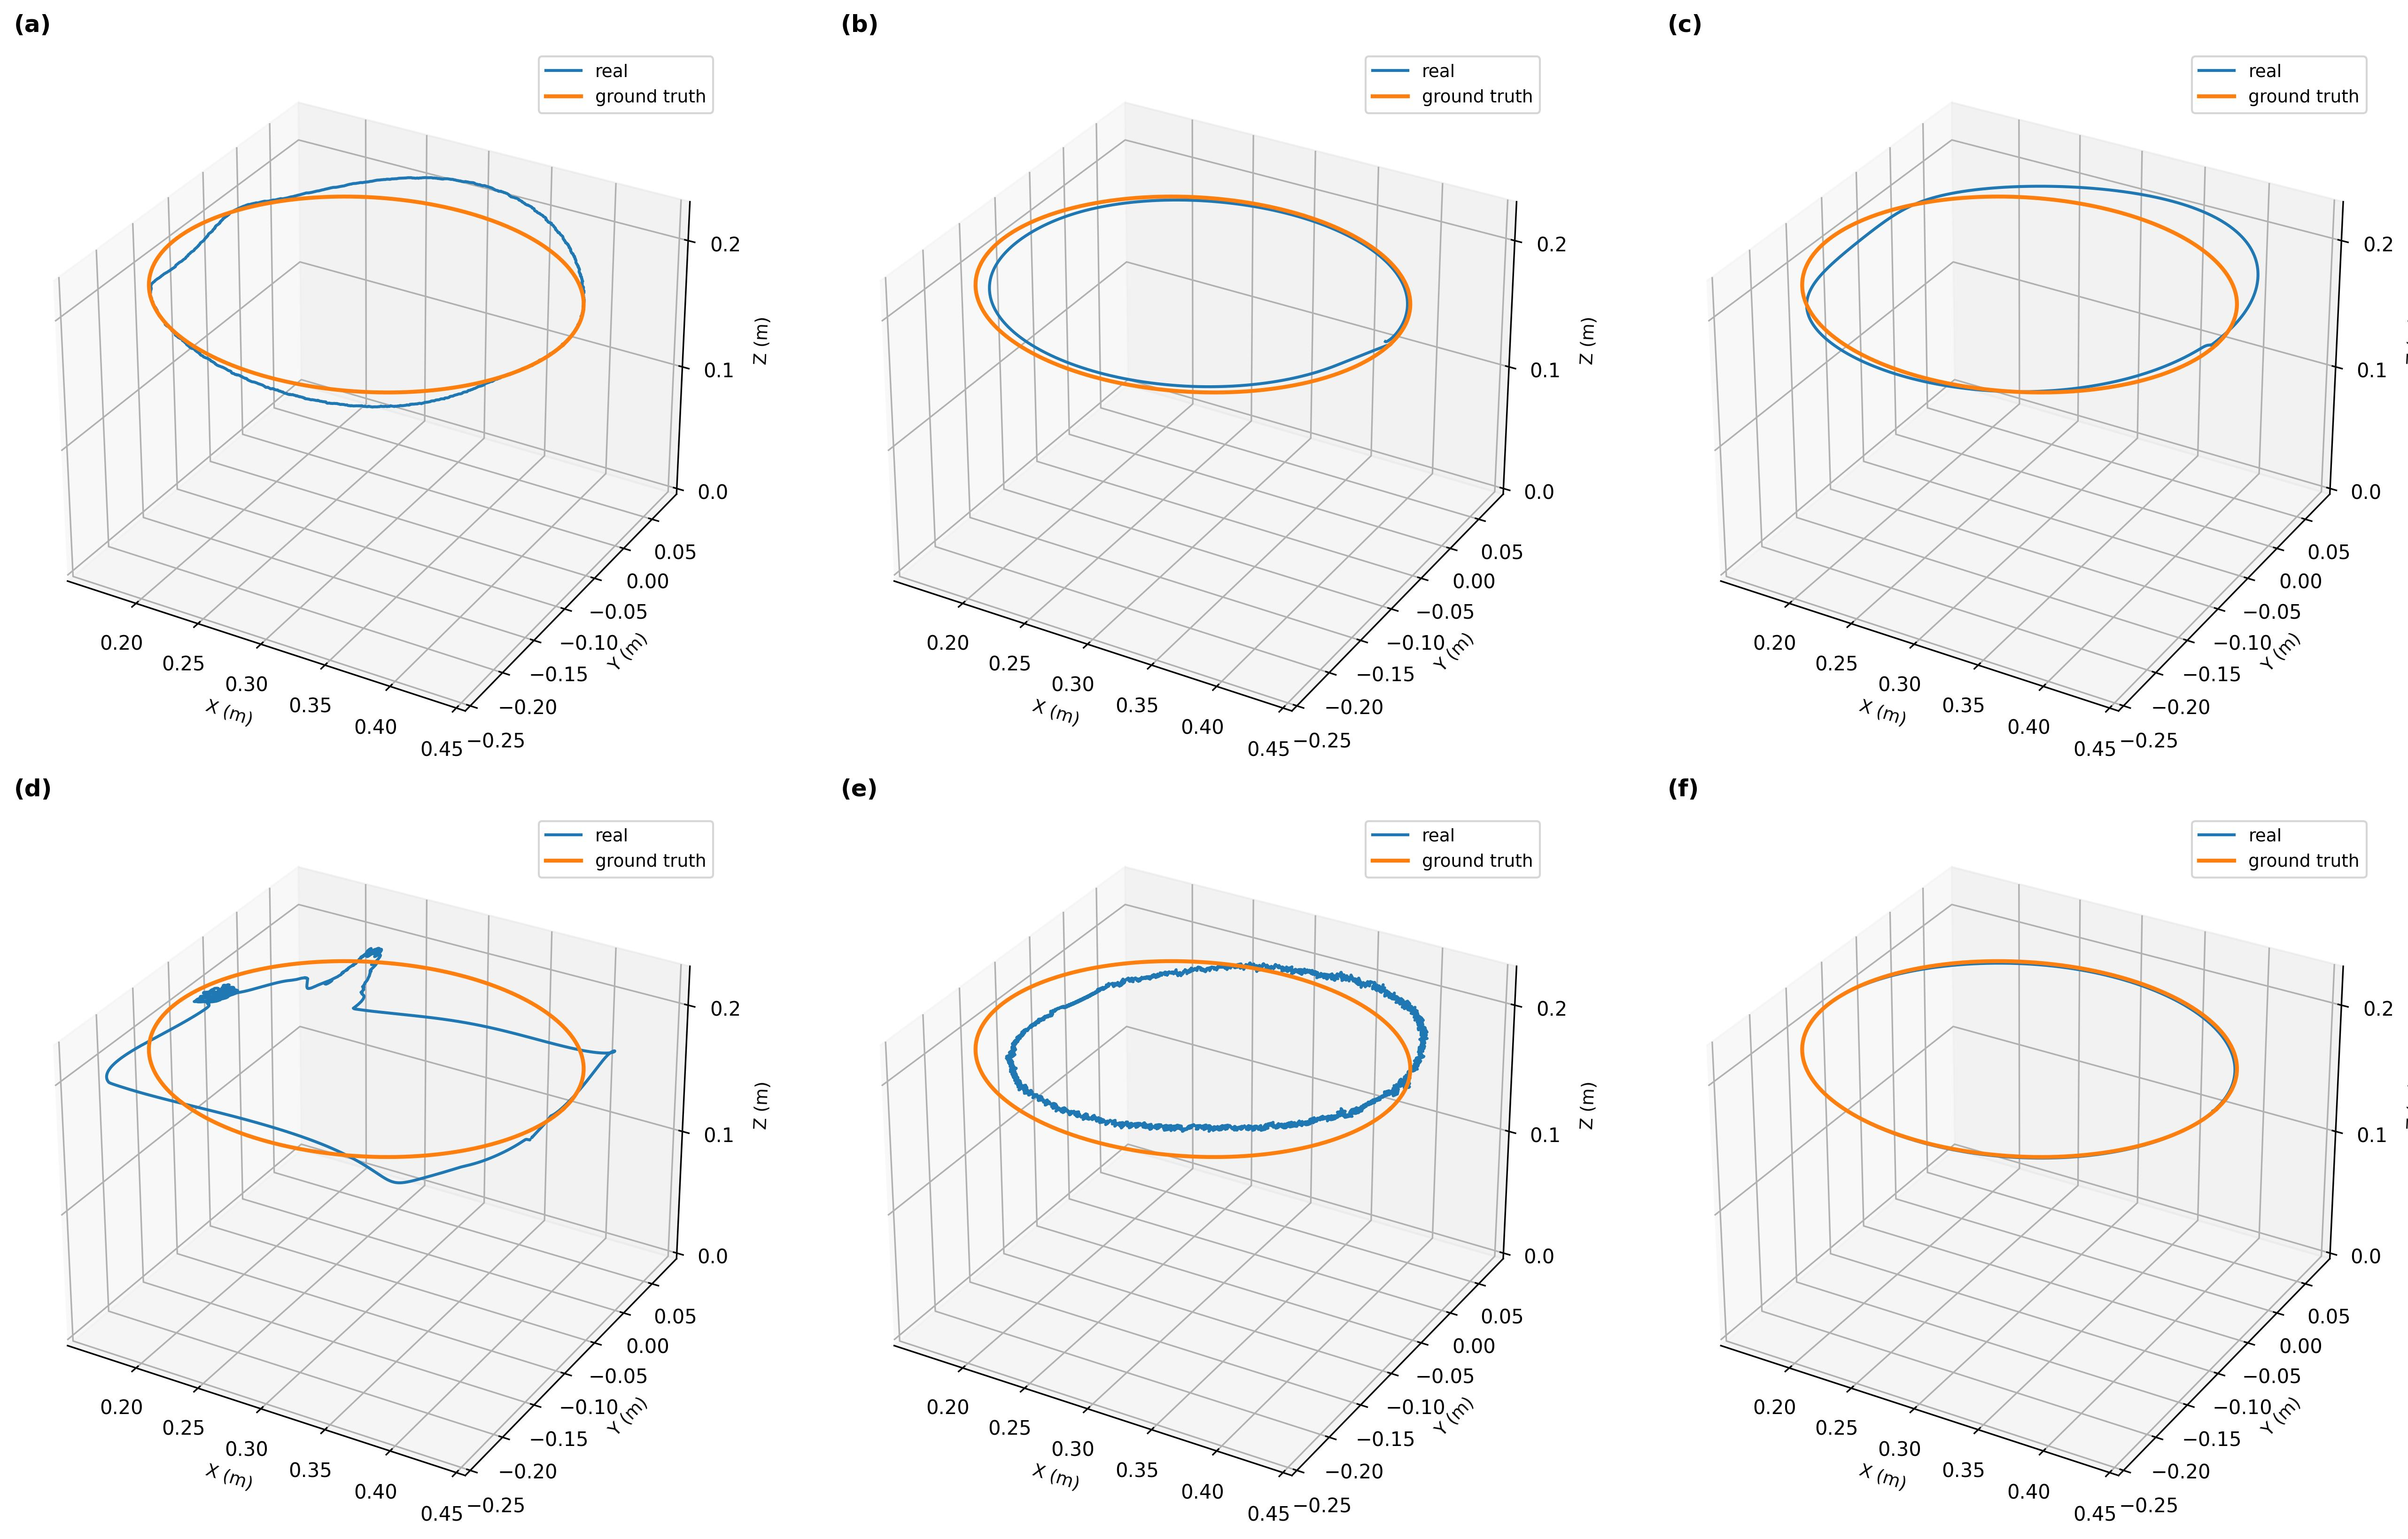
\includegraphics[width=\linewidth]{circle.jpg}
    \caption{Circle Trajectory Comparison (a) TRAC-IK (b) DLS Pseudo Inverse Jacobian (c) Velocity QP (d) TRPO-D (e) SAC-S (f) PPO-D}
    \label{fig:plots_comparison}
\end{figure}
% \begin{figure}
%     \centering
%     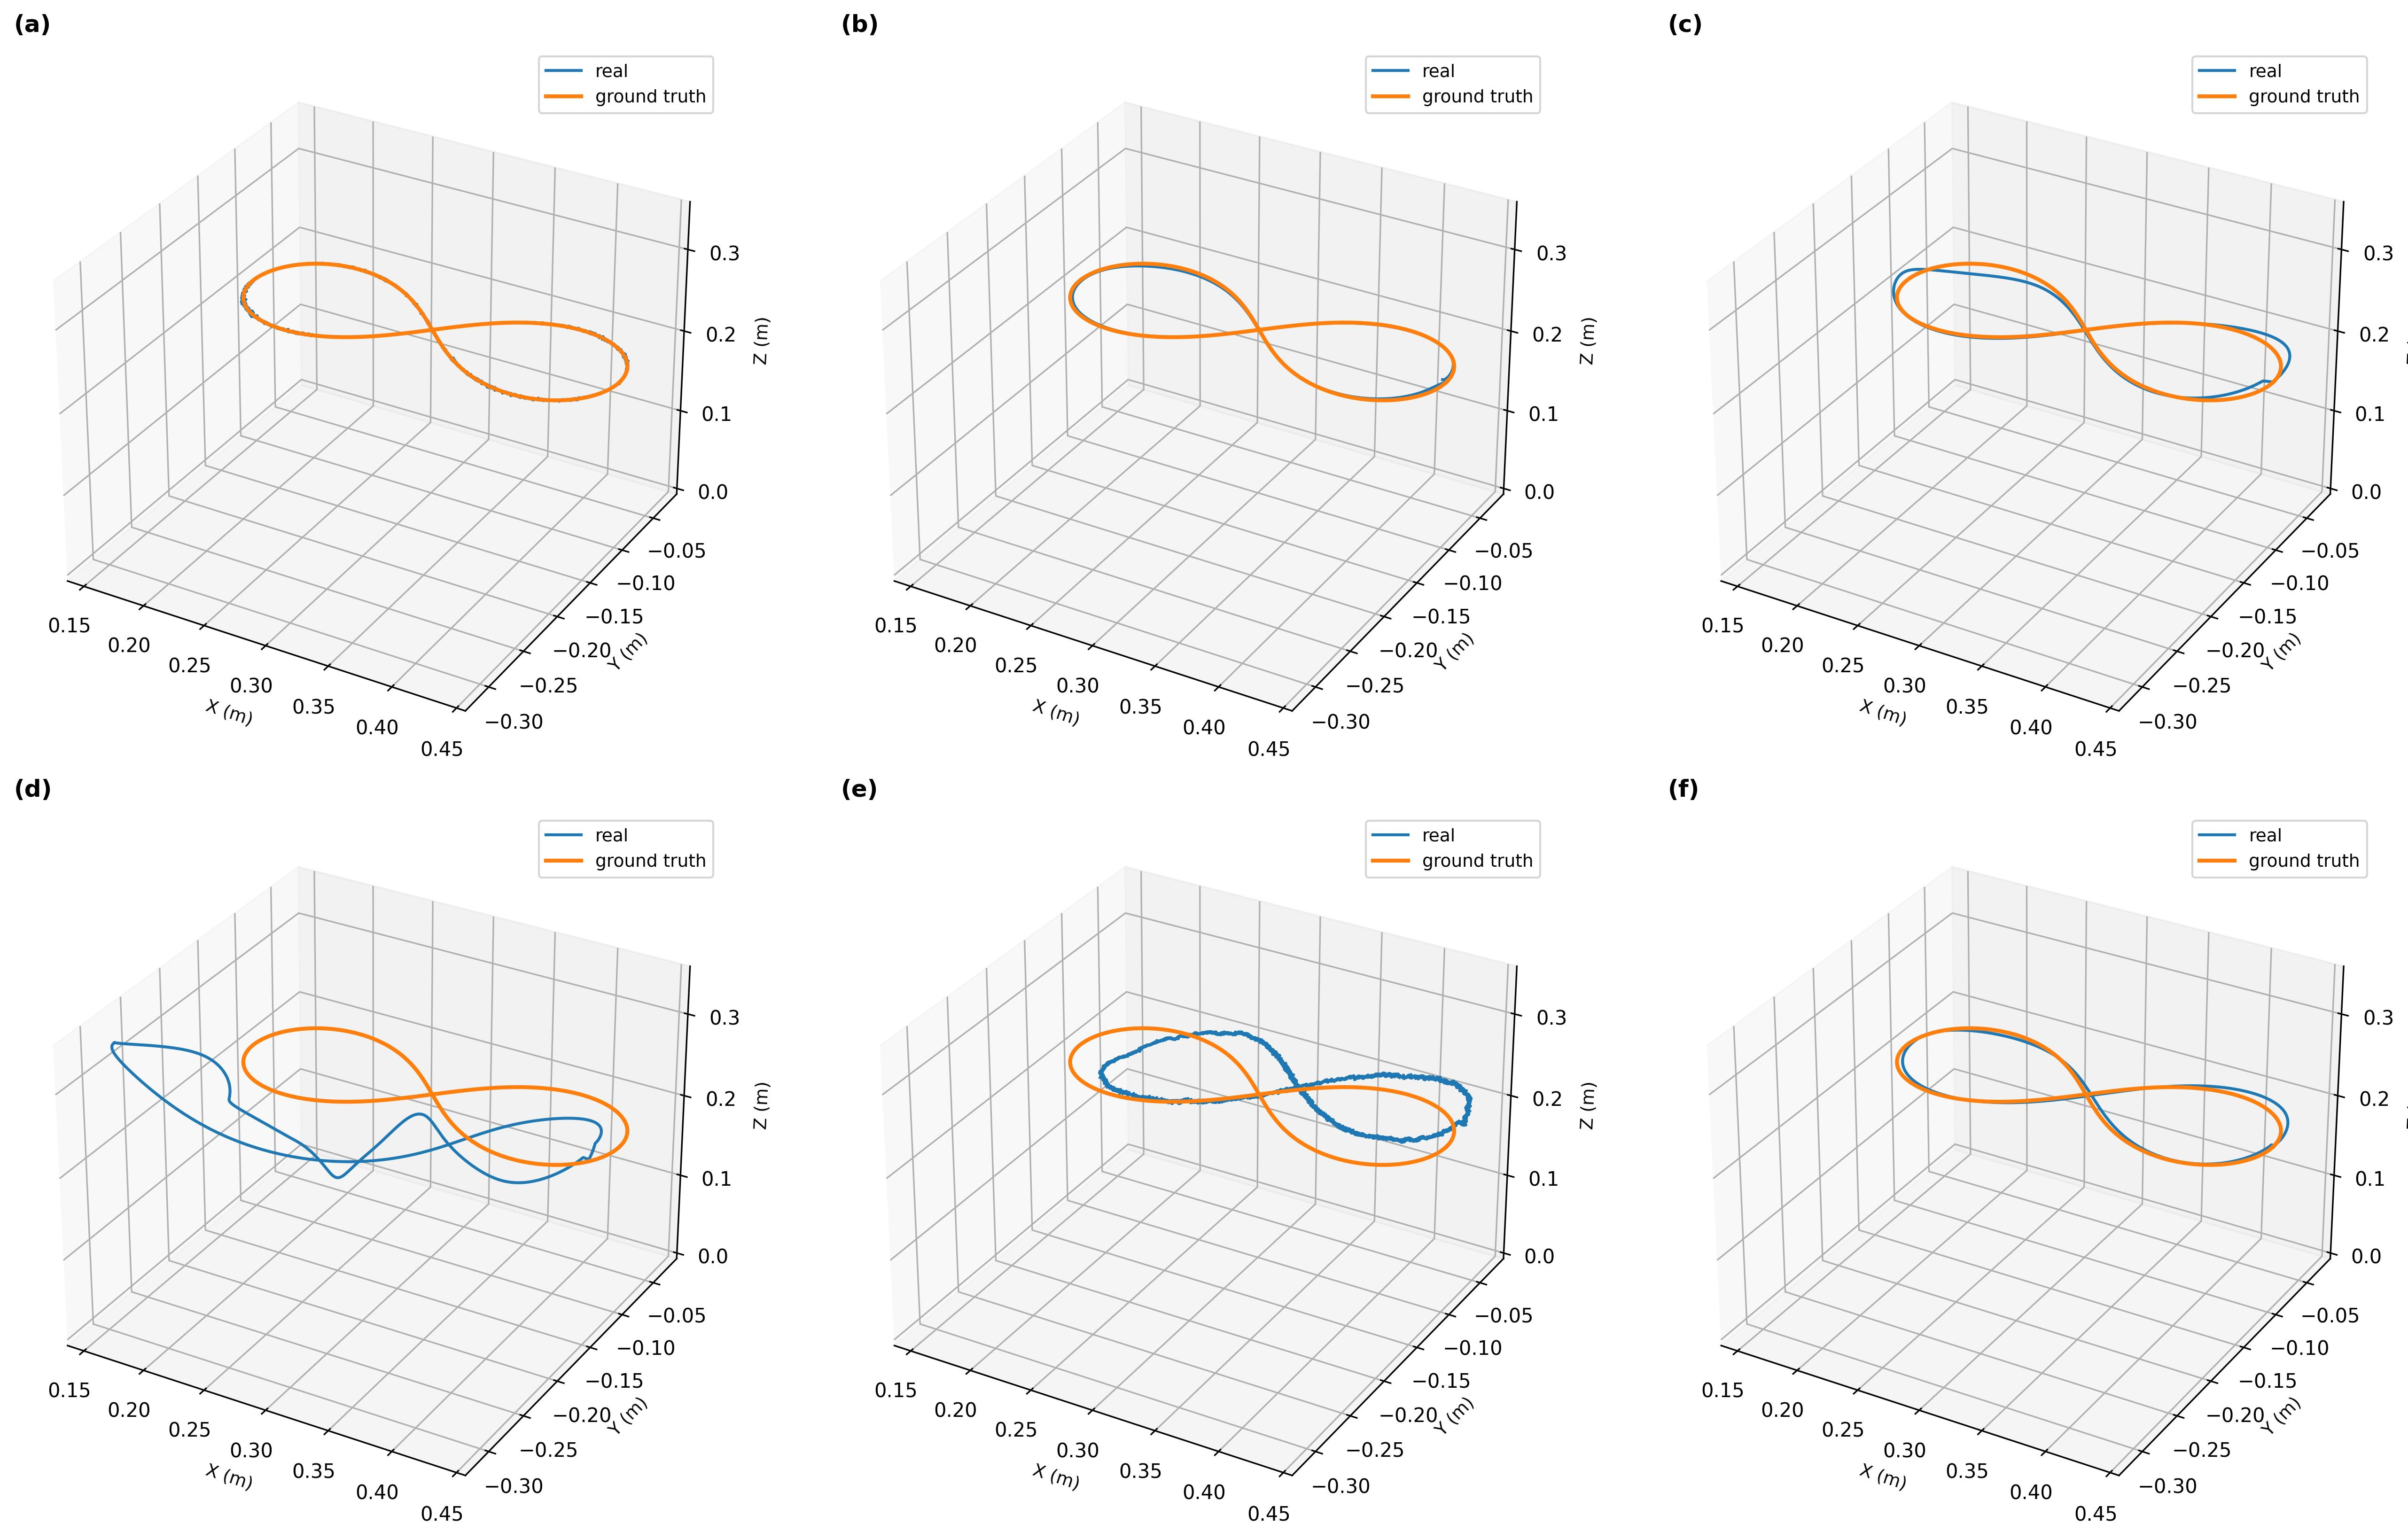
\includegraphics[width=\linewidth]{lemniscate.jpg}
%     \caption{3-D Lemniscate Trajectory Comparison (a) TRAC-IK (b) DLS Pseudo Inverse Jacobian (c) Velocity QP (d) TRPO-D (e) SAC-S (f) PPO-D}
%     \label{fig:plots_comparison_1}
% \end{figure}
\begin{figure}
    \centering
    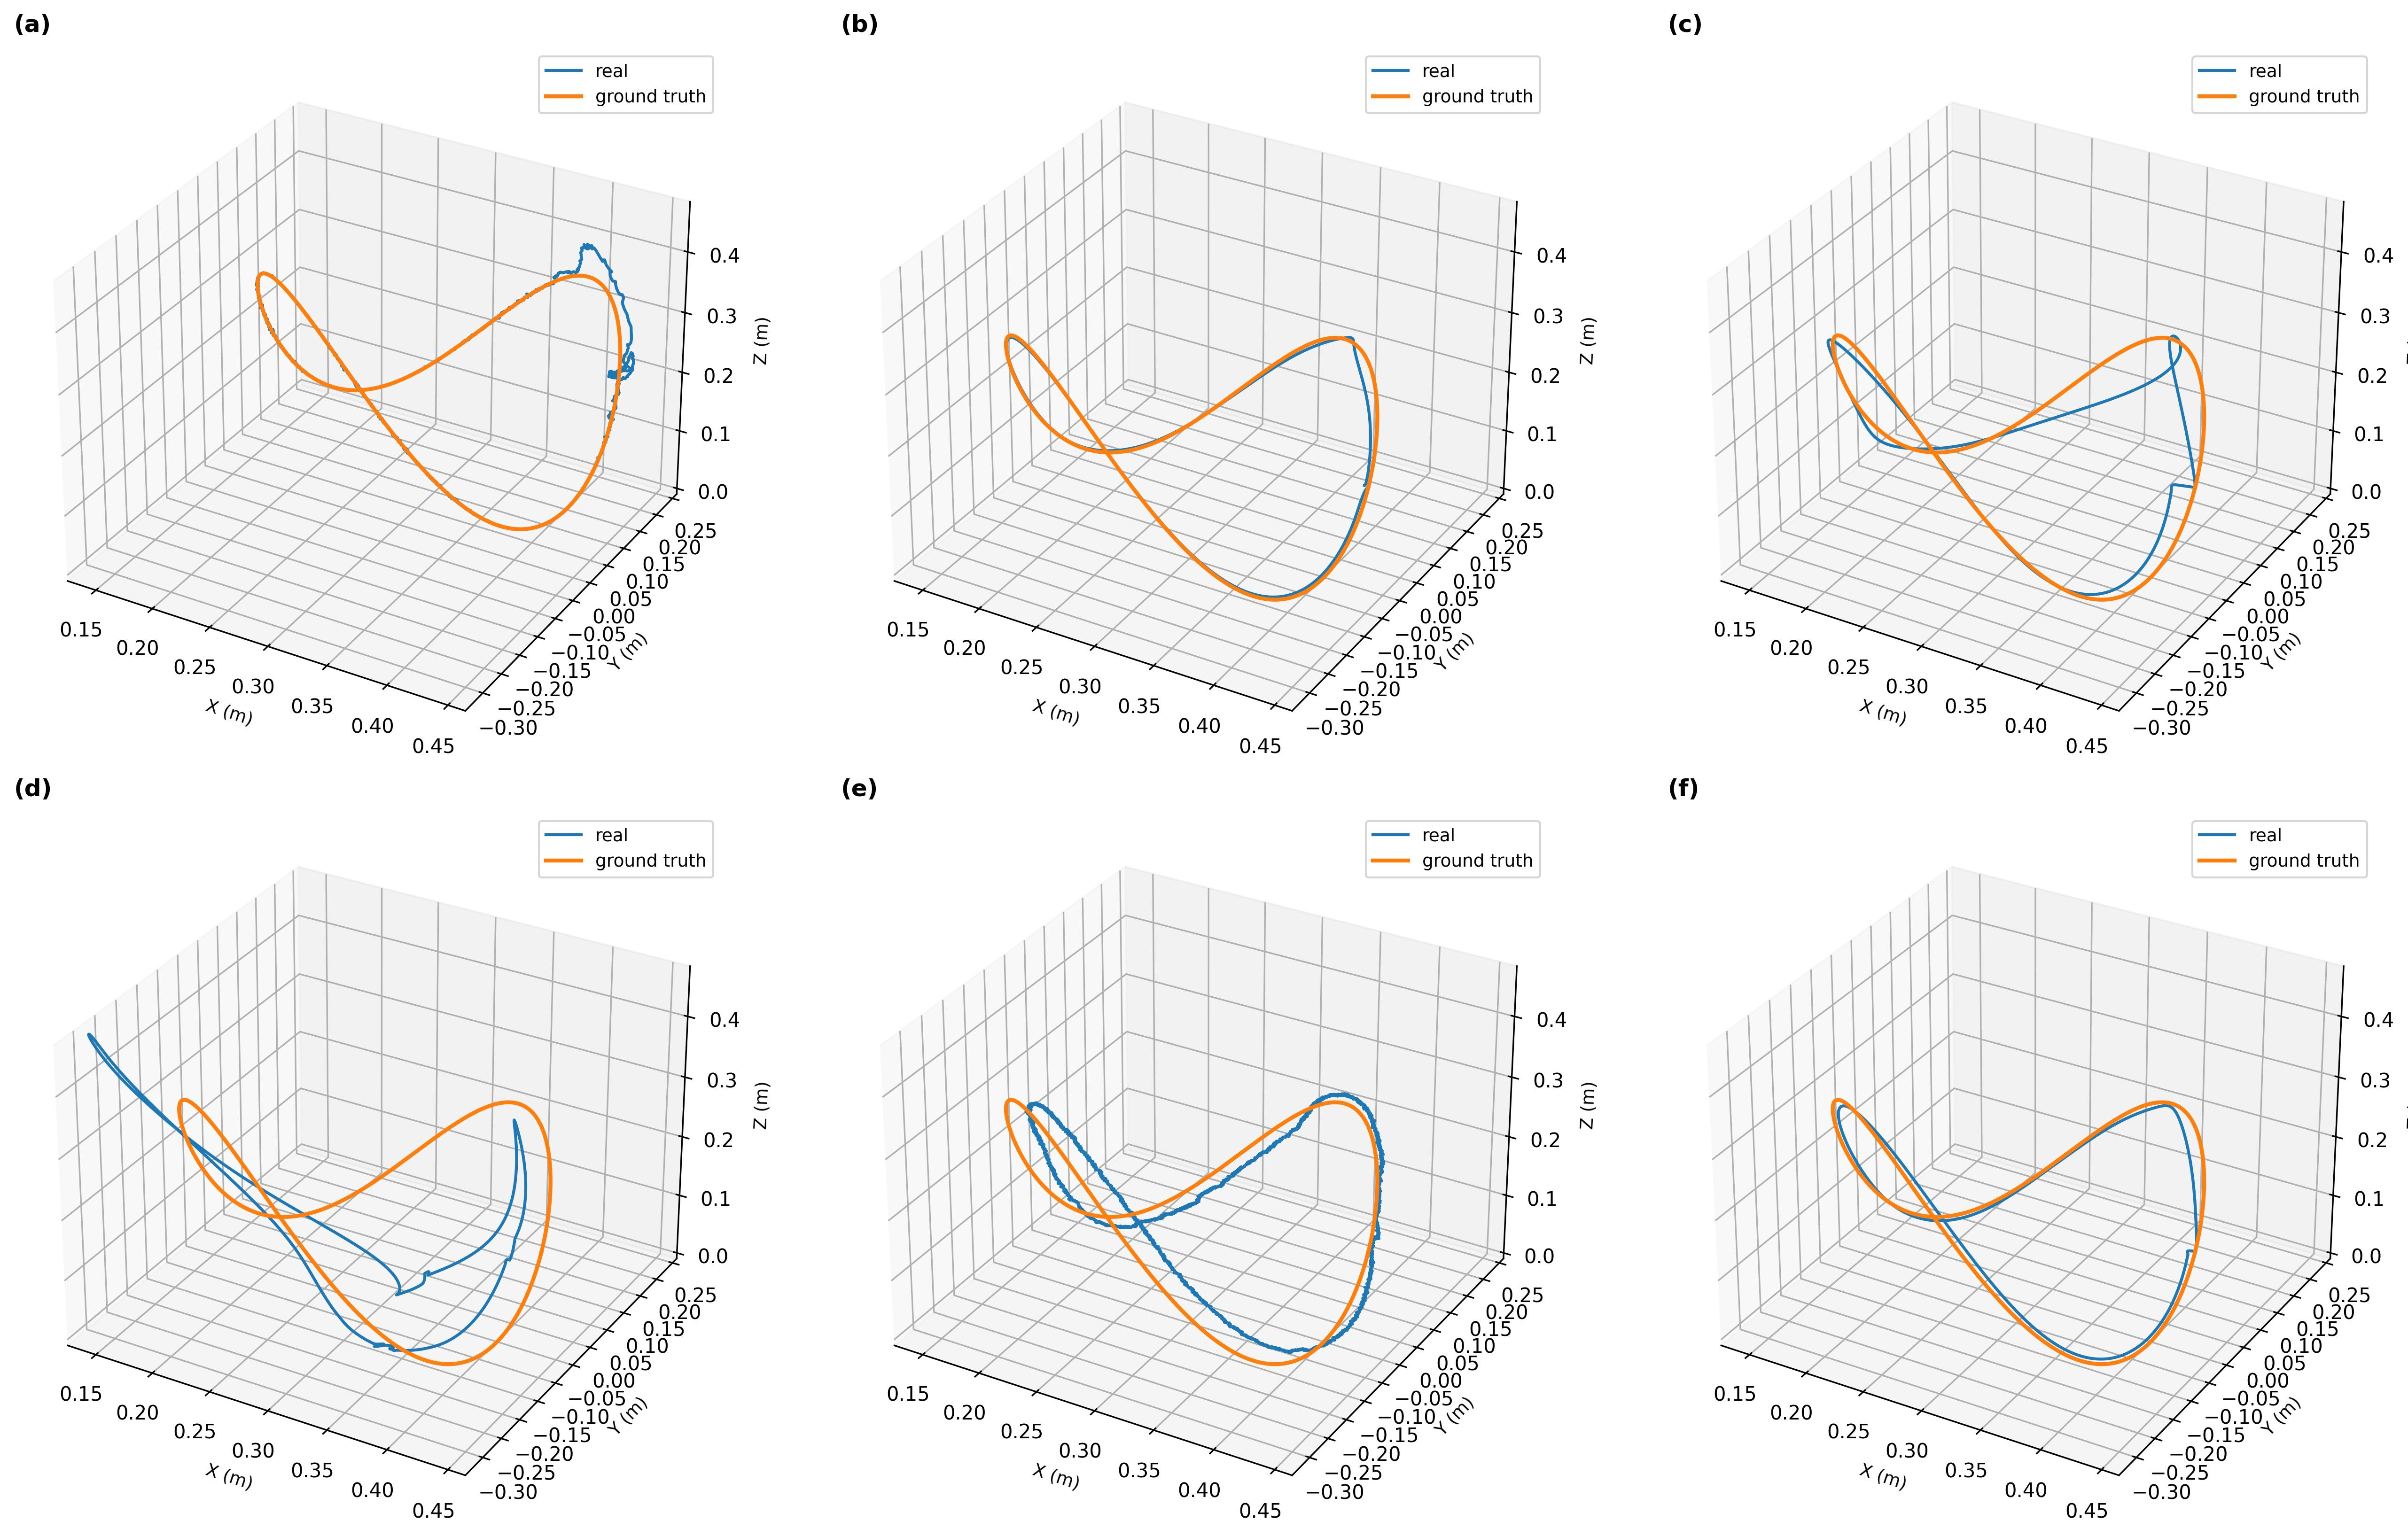
\includegraphics[width=\linewidth]{lissajous.jpg}
    \caption{3-D Lissajous Trajectory Comparison (a) TRAC-IK (b) DLS Pseudo Inverse Jacobian (c) Velocity QP (d) TRPO-D (e) SAC-S (f) PPO-D}
    \label{fig:plots_comparison_2}
\end{figure}
% \begin{figure}
%     \centering
%     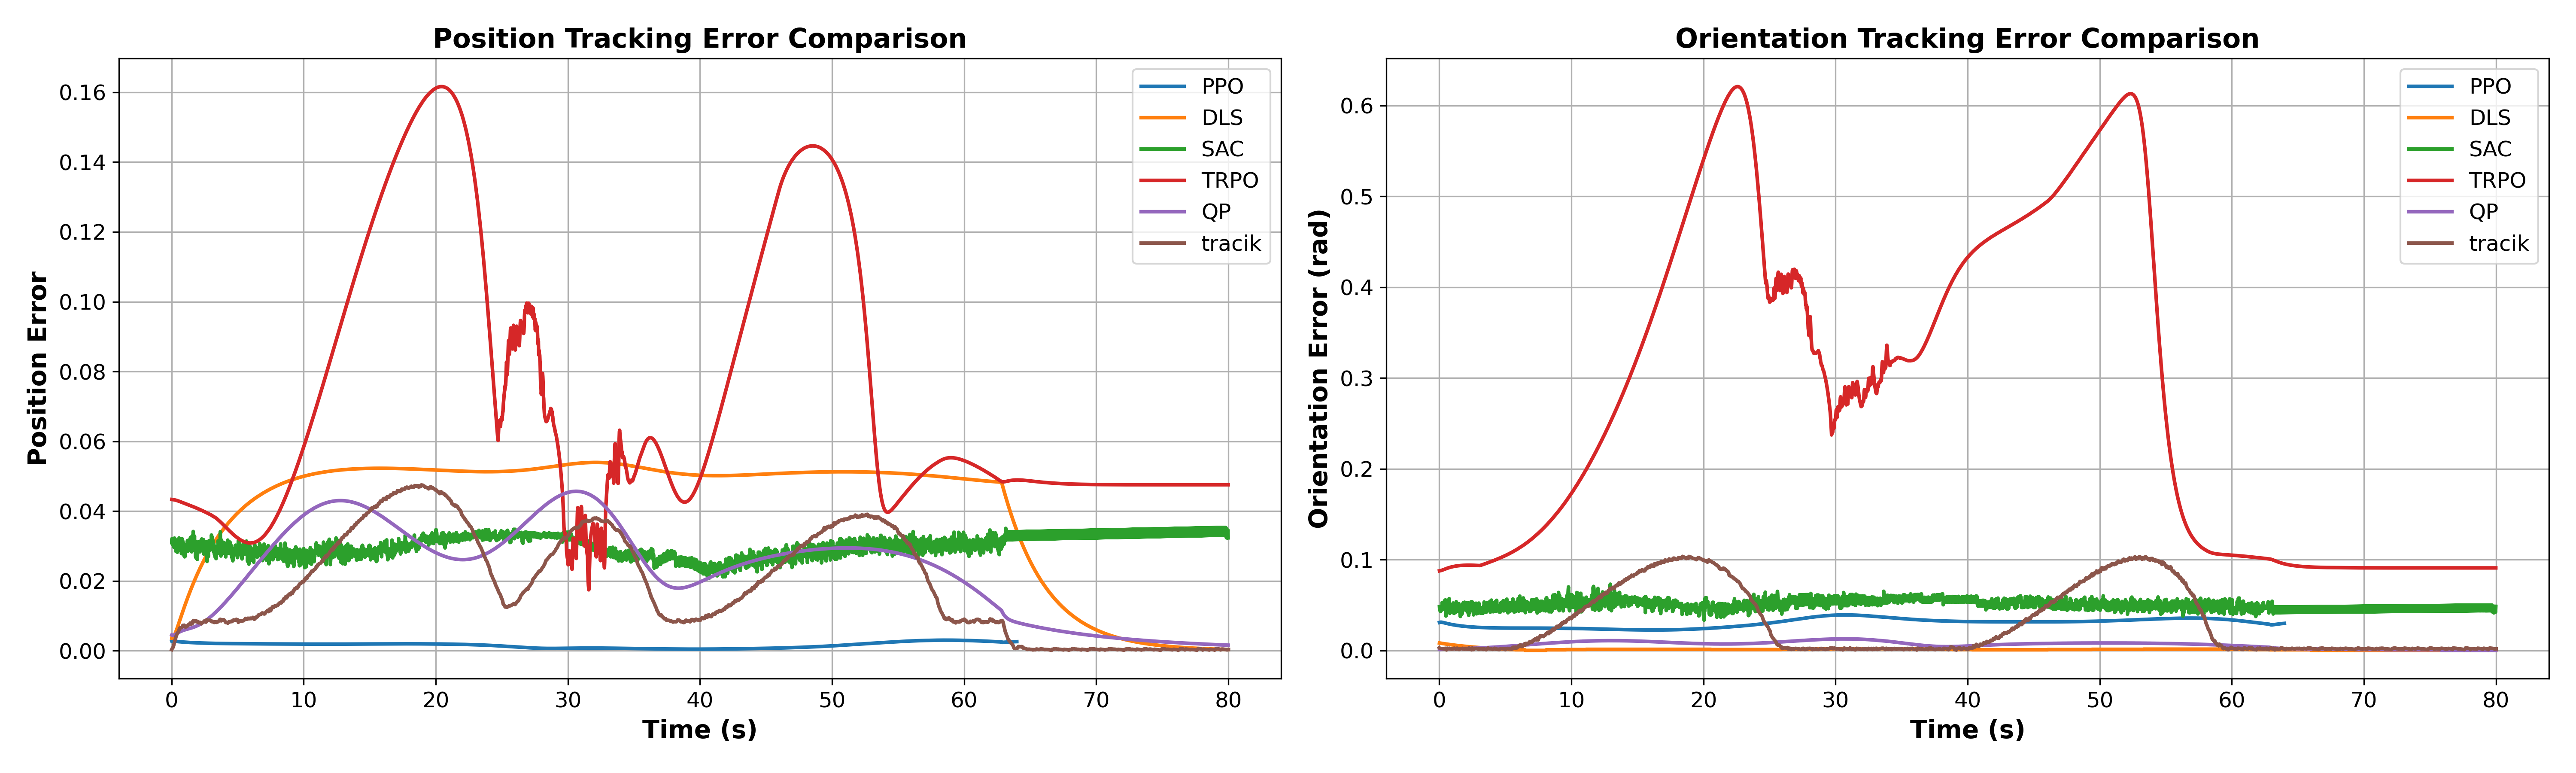
\includegraphics[width=\linewidth]{Fig_9.png}
%     \caption{Pose Tracking Error Comparisons across Existing Methods in Simulation}
%     \label{fig:pose_track_error_sim}
% \end{figure}
%%%%%%%%%%%%%%%%%%
\begin{table*}[h]
\centering
\caption{Simulation performance across circle, lemniscate, and 3-D
Lissajous trajectories with frozen per-method action scales
(Section~4.1). No classical baseline is uniformly best; PPO is the only
method with stable accuracy and smoothness across all three geometries.
Best value per metric in bold.}
\label{tab:performance_comparison}
\renewcommand{\arraystretch}{1.0}
\setlength{\tabcolsep}{3pt}
\begin{tabular}{llcccc}
\toprule
\textbf{Method} & \textbf{Curve} & $\mathbf{a_{\mathrm{scale}}}$ & \textbf{Pos. RMSE} $\downarrow$ & \textbf{Orn. RMSE} $\downarrow$ & \textbf{Smoothness} $\downarrow$ \\
\midrule

\multirow{3}{*}{Trac-IK}
& Circle      & 0.2 & 0.001242 & 0.003409 & 54.547754 \\
& Lemniscate  & 0.2 & \textbf{0.001073} & 0.004332 & 52.002110 \\
& Lissajous   & 0.2 & 0.035272 & 0.052286 & 62.164647 \\

\midrule

\multirow{3}{*}{DLS}
& Circle      & 1 & 0.016046 & \textbf{0.000767} & 0.013438 \\
& Lemniscate  & 1 & 0.013554 & 0.036097 & 0.015920 \\
& Lissajous   & 1 & 0.027939 & 0.020683 & 0.022242 \\

\midrule

\multirow{3}{*}{Vel QP}
& Circle      & 1 & 0.011013 & 0.002900 & 0.012409 \\
& Lemniscate  & 1 & 0.013254 & 0.003857 & 0.029433 \\
& Lissajous   & 1 & 0.035303 & 0.008647 & 0.016406 \\

\midrule

\multirow{3}{*}{TRPO}
& Circle      & 0.4 & 0.089448 & 0.372891 & 2.918600 \\
& Lemniscate  & 0.4 & 0.130428 & 0.383532 & 0.141100 \\
& Lissajous   & 0.4 & 0.122329 & 0.257595 & 0.814877 \\

\midrule

\multirow{3}{*}{SAC}
& Circle      & 0.2 & 0.029320 & 0.051513 & 19.778952 \\
& Lemniscate  & 0.2 & 0.030142 & 0.051104 & 19.077041 \\
& Lissajous   & 0.2 & 0.029181 & 0.050908 & 18.851007 \\

\midrule

\multirow{3}{*}{PPO}
& Circle      & 1 & 0.009951 & 0.026476 & \textbf{0.005545} \\
& Lemniscate  & 1 & 0.010650 & 0.023536 & 0.010719 \\
& Lissajous   & 1 & 0.016667 & 0.043686 & 0.014745 \\

\bottomrule
\label{tab:error_metrics_sim}
\end{tabular}
\end{table*}
%%%%%%%%%%%%%%%%%%
% \begin{table}[h]
% \centering
% \caption{Simulation Circular Trajectory Tracking Performance Comparisons(*\textit{best results are bold})} 
% \label{tab:error_metrics_sim}
% \begin{tabular}{lccccc}
% \midrule
% \textbf{Method} & \textbf{Pos RMSE(m)} & \textbf{Orn RMSE(rad)}\\
% \midrule\midrule
% TRAC-IK & $2.7\times 10^{-2}$ & $5.4 \times 10^{-2}$\\
% DLS & $4.8\times 10^{-2}$ & $\boldsymbol{1.6 \times 10^{-3}}$\\
% QP & $2.9\times 10^{-2}$ & $7.9 \times 10^{-3}$ \\
% TRPO & $8.9\times 10^{-2}$ & $3.7 \times 10^{-1}$\\
% SAC-S & $2.9\times 10^{-2}$ & $5.1 \times 10^{-2}$\\
% PPO-D & $ \boldsymbol{1.7\times 10^{-3}}$ & $3.0 \times 10^{-2}$\\
% \midrule
% \end{tabular}
% \end{table}
No single classical baseline is uniformly best, and the pattern of
failure for each is a direct consequence of its underlying mechanism
rather than a tuning artifact.

TRAC-IK resolves each waypoint as an independent constrained
optimization, seeded by the previous joint state. In a noiseless
simulation this allows near-exact convergence at every individual pose,
producing the lowest position RMSE among all methods on the circle
(1.2~mm) and lemniscate (1.07~mm), Tab~\ref{tab:error_metrics_sim}. However, because each solve is independent with no explicit velocity-domain coupling between consecutive timesteps, small differences in optimizer convergence translate directly into joint-space discontinuities frame-to-frame. This is the mechanistic cause of its smoothness index of (52--62), three to four orders of magnitude worse than every other method. On the Lissajous trajectory, where curvature and orientation change, the nearest-seed assumption that keeps TRAC-IK well-behaved on planar curves breaks down, and the solver begins to favor configuration branches discontinuous with the previous solution, position RMSE degrades by roughly 30$\times$ (1.2~mm $\rightarrow$ 35.3~mm) relative to the circle.

DLS computes joint velocities from a damped pseudo-inverse Jacobian with
a fixed damping factor $\lambda = 0.05$ and a single, undifferentiated
gain applied to the combined position-orientation error vector. On the
circle, where orientation is held constant, this fixed gain structure
strongly favors orientation correction, since the magnitude of angular
correction required to track a fixed orientation is small and well within
the controller's effective bandwidth, yielding the best orientation RMSE
of any method (7.7$\times10^{-4}$~rad) at the cost of a comparatively
large 16~mm position error. On the lemniscate, where orientation must
vary continuously alongside position, the same fixed gain cannot
adaptively reallocate correction authority between the two error
channels, and orientation RMSE rises to 0.036~rad, worse than the
proposed method's 0.024~rad on the identical curve. DLS's strong circle
orientation result is therefore a constant-orientation artifact of its
fixed-gain structure, not a general advantage over learned methods.

Velocity QP imposes the same differential-Jacobian structure as DLS but
adds explicit joint-limit constraints via sequential quadratic programming. It sits between DLS and TRAC-IK in position accuracy across all three curves (11.0--35.3~mm) without leading on any single metric, consistent with QP correcting DLS's joint-limit violations without altering DLS's fundamental fixed-gain error-coupling. 

TRPO shares PPO's coupled reward (Eq.~\ref{final_pose_reward}, Eq.~\ref{progress_reward}, Eq.~\ref{energy_penalty}) and its on-policy,
trust-region-constrained update rule, but enforces an exact KL-divergence
constraint rather than PPO's clipped surrogate objective. The exact
constraint requires a more expensive constrained optimization step per
update; under an identical training budget (Tab~\ref{tab:ppo_hyperparams}), this leaves TRPO's
policy less converged than PPO's at the same total timestep count,
producing both higher residual position/orientation error (8.9~cm /
0.37~rad on the circle) and substantially worse smoothness on the circle
(2.92) than PPO (0.0055), since incomplete convergence leaves residual
policy stochasticity in the action distribution.

SAC optimizes a maximum-entropy objective that explicitly rewards
maintaining stochasticity in the action distribution. This directly
conflicts with the exponential energy penalty (Eq.~\ref{energy_penalty}), which penalizes any nonzero joint velocity once near convergence. The two objectives admit a stable compromise in which the policy sustains a small, persistent non-zero error rather than fully converging, since fully converging would require collapsing the action entropy that the SAC objective rewards. This is visible as a consistent radial offset of $\approx$2.9~cm on the circle and a smoothness index of 18.9--19.8 across all three curves, essentially unchanged by trajectory geometry, which is itself consistent with the offset being an artifact of the entropy-energy trade-off rather than a tracking failure specific to any one curve.

PPO does not achieve the lowest position RMSE in simulation on every
curve; rather, it is the most consistent method across geometries, with
position RMSE confined to a 9.9--16.7~mm band across circle, lemniscate,
and Lissajous, while every classical baseline degrades sharply on at
least one curve (TRAC-IK by $\sim$30$\times$ on Lissajous; DLS's
orientation by $\sim$47$\times$ on lemniscate). PPO is also the smoothest
method by one to four orders of magnitude on every curve
(0.0055--0.0147 versus 0.012--62.2 for the baselines).

This consistency is not an incidental property of PPO as an algorithm;
it follows directly from the structure of the proposed reward. The
min-operator coupling in Eq.~\ref{final_pose_reward} prevents the policy from trading orientation accuracy for position accuracy under the shifting demands of each curve, which is why PPO does not exhibit the orientation collapse seen in DLS on the lemniscate, where position and orientation
requirements vary continuously rather than remaining fixed as on the
circle. The asymmetric progress shaping in Eq.~\ref{progress_cond} penalizes stagnation at every timestep regardless of trajectory geometry, consistent with PPO avoiding both the persistent radial offset exhibited by SAC and the oscillatory non-convergence exhibited by TRAC-IK and QP, since both behaviors correspond to sustained, under-penalized error under a sparser or differently-structured reward. The exponential energy penalty in Eq.~\ref{energy_penalty} acts directly on joint velocity magnitude, which is the proximate cause of PPO's smoothness advantage over every baseline, independent of trajectory shape. None of the classical baselines or alternative RL baselines (TRPO, SAC) share this reward structure, which is why their performance is uneven across geometries while PPO's is not. The contribution is therefore the reward formulation itself; the choice of
PPO as the optimizer is a secondary, empirically justified design
decision (Sec~\ref{reward_ablation}), not the source of the result.





% TRPO~(Fig.~\ref{fig:plots_comparison}(d)) exhibits severe trajectory deviation with sharp angular deviations, with respective degraded RMSE of 0.089~m and 0.37~rad in position and orientation respectively Tab~\ref{tab:error_metrics_sim}. SAC-S(e) completes the trajectory with a consistent radial offset, reflected in a steady $\approx$0.029~m position error throughout, comparable to TRAC-IK. Among the classical methods, DLS(b) achieves strict orientation tracking ($\approx$0.0016~rad RMSE) but at the cost of $\approx$0.05~m position drift through the trajectory. TRAC-IK and QP track the trajectory visually but oscillate around $\approx$0.03~m without converging. PPO-D(f) achieves a near-perfect trajectory overlap with ground truth, sustained near position error throughout 80 seconds, and the better position RMSE of 0.0017~m compared to all remaining  baselines.
\subsection{Real-time Results}
\label{real_time_deployment}
The same circular, square, lemniscate, and 3-D Lissajous trajectories
used in simulation (Section~4.1) are evaluated on hardware. All trajectories execute at 20~Hz closed-loop frequency, using the same trajectory parameters as in simulation ($r = 0.15$~m, center $[0.3, -0.1, 0.2]$~m, angular velocity $0.1$~rad/s). TRAC-IK, DLS, and SAC are validated on hardware for the circular trajectory~(Fig.~\ref{fig:extra-real}), one representative baseline per method family (classical numerical, classical velocity-level, and RL), while the proposed method is further evaluated on lemniscate, 3-D Lissajous, and square trajectories~(Fig.~\ref{real_trajec_const_orientation}, Fig.~\ref{real_trajec_var_orientation}). Velocity QP is omitted from the hardware comparison, as its simulation behavior does not differentiate it from DLS along any metric that would justify an additional hardware trial. The error metrics observed of this study are listed in Tab~\ref{tab:error_metrics_real}.
\begin{figure}
    \centering
    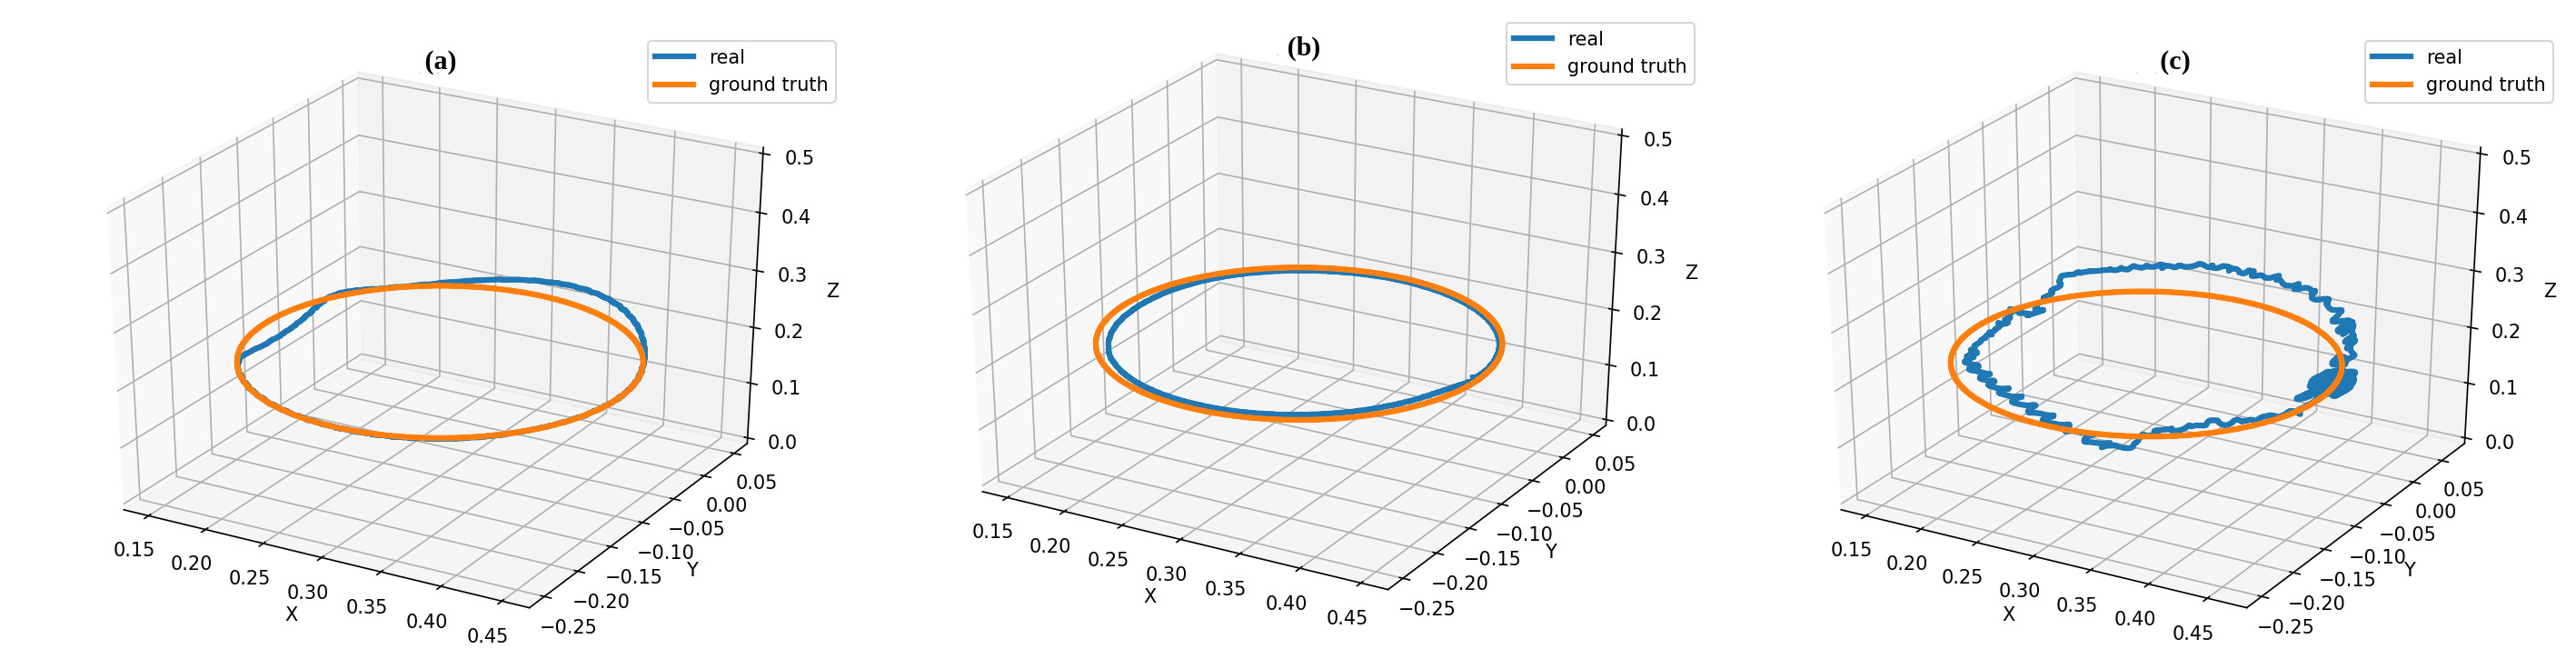
\includegraphics[width=\linewidth]{Fig_13.jpg}
    \caption{Real-time Deployment of (a) TRAC-IK (b) DLS (c) SAC-S}
    \label{fig:extra-real}
\end{figure}
\begin{figure}
    \centering
    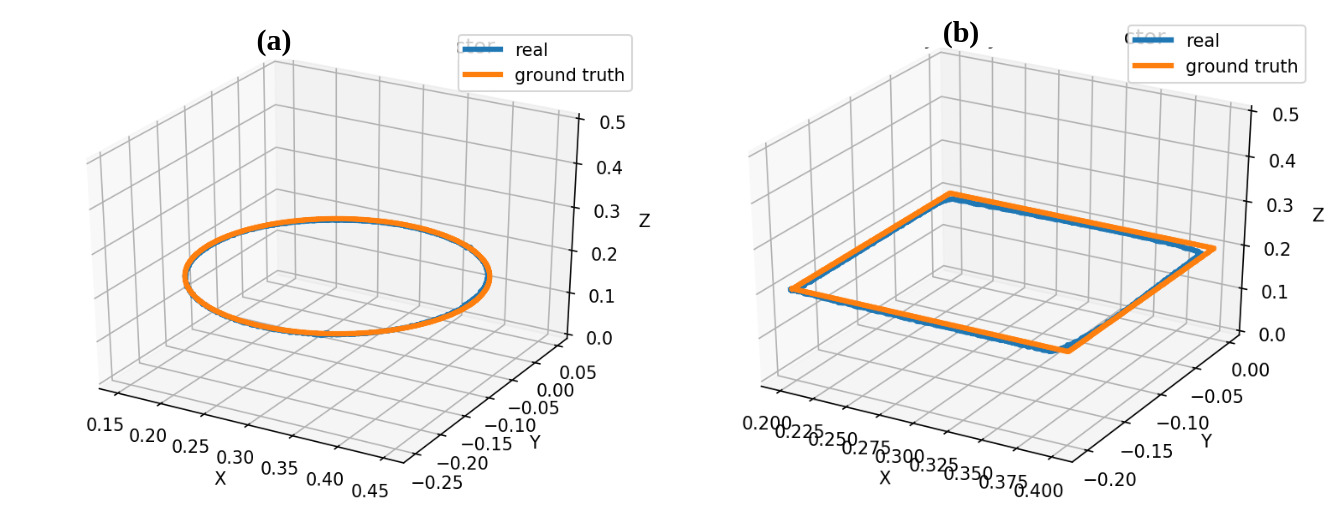
\includegraphics[width=\linewidth]{Fig_10.jpg}
    \caption{Real-Time Trajectory tracking of (a) Circle (b) Square with constant end effector orientation.}
    \label{real_trajec_const_orientation}
\end{figure}
\begin{figure}
    \centering
    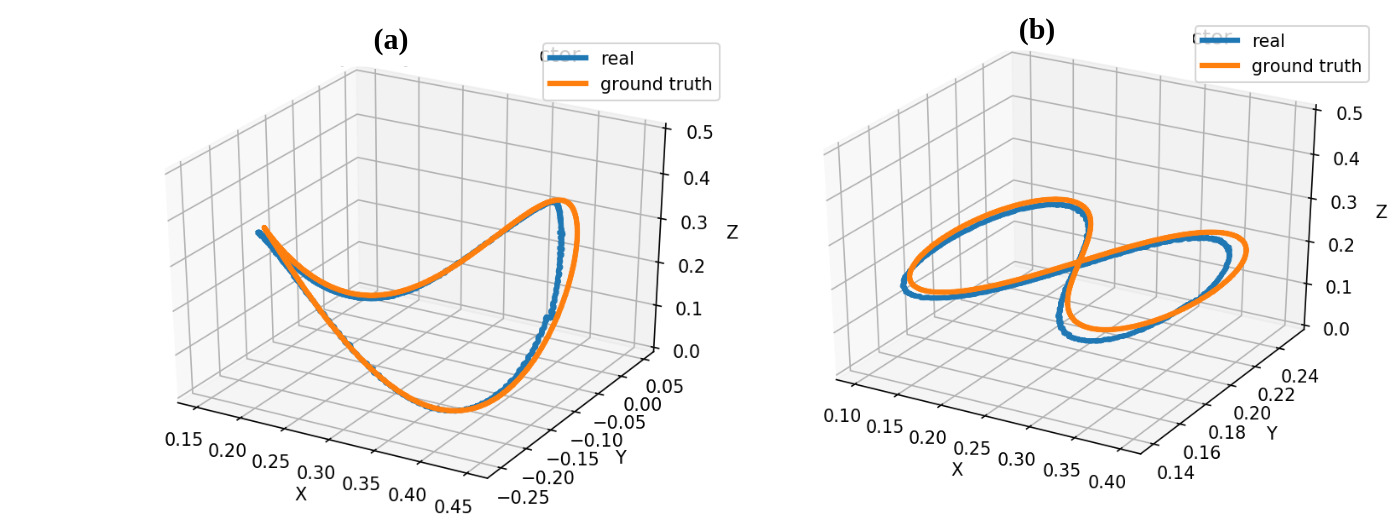
\includegraphics[width=\linewidth]{Fig_11.jpg}
    \caption{Real-Time Trajectory tracking of (a) 3-D Lissajous (b) Lemniscate with varying end effector orientation.}
    \label{real_trajec_var_orientation}
\end{figure}
% \begin{figure}
%     \centering
%     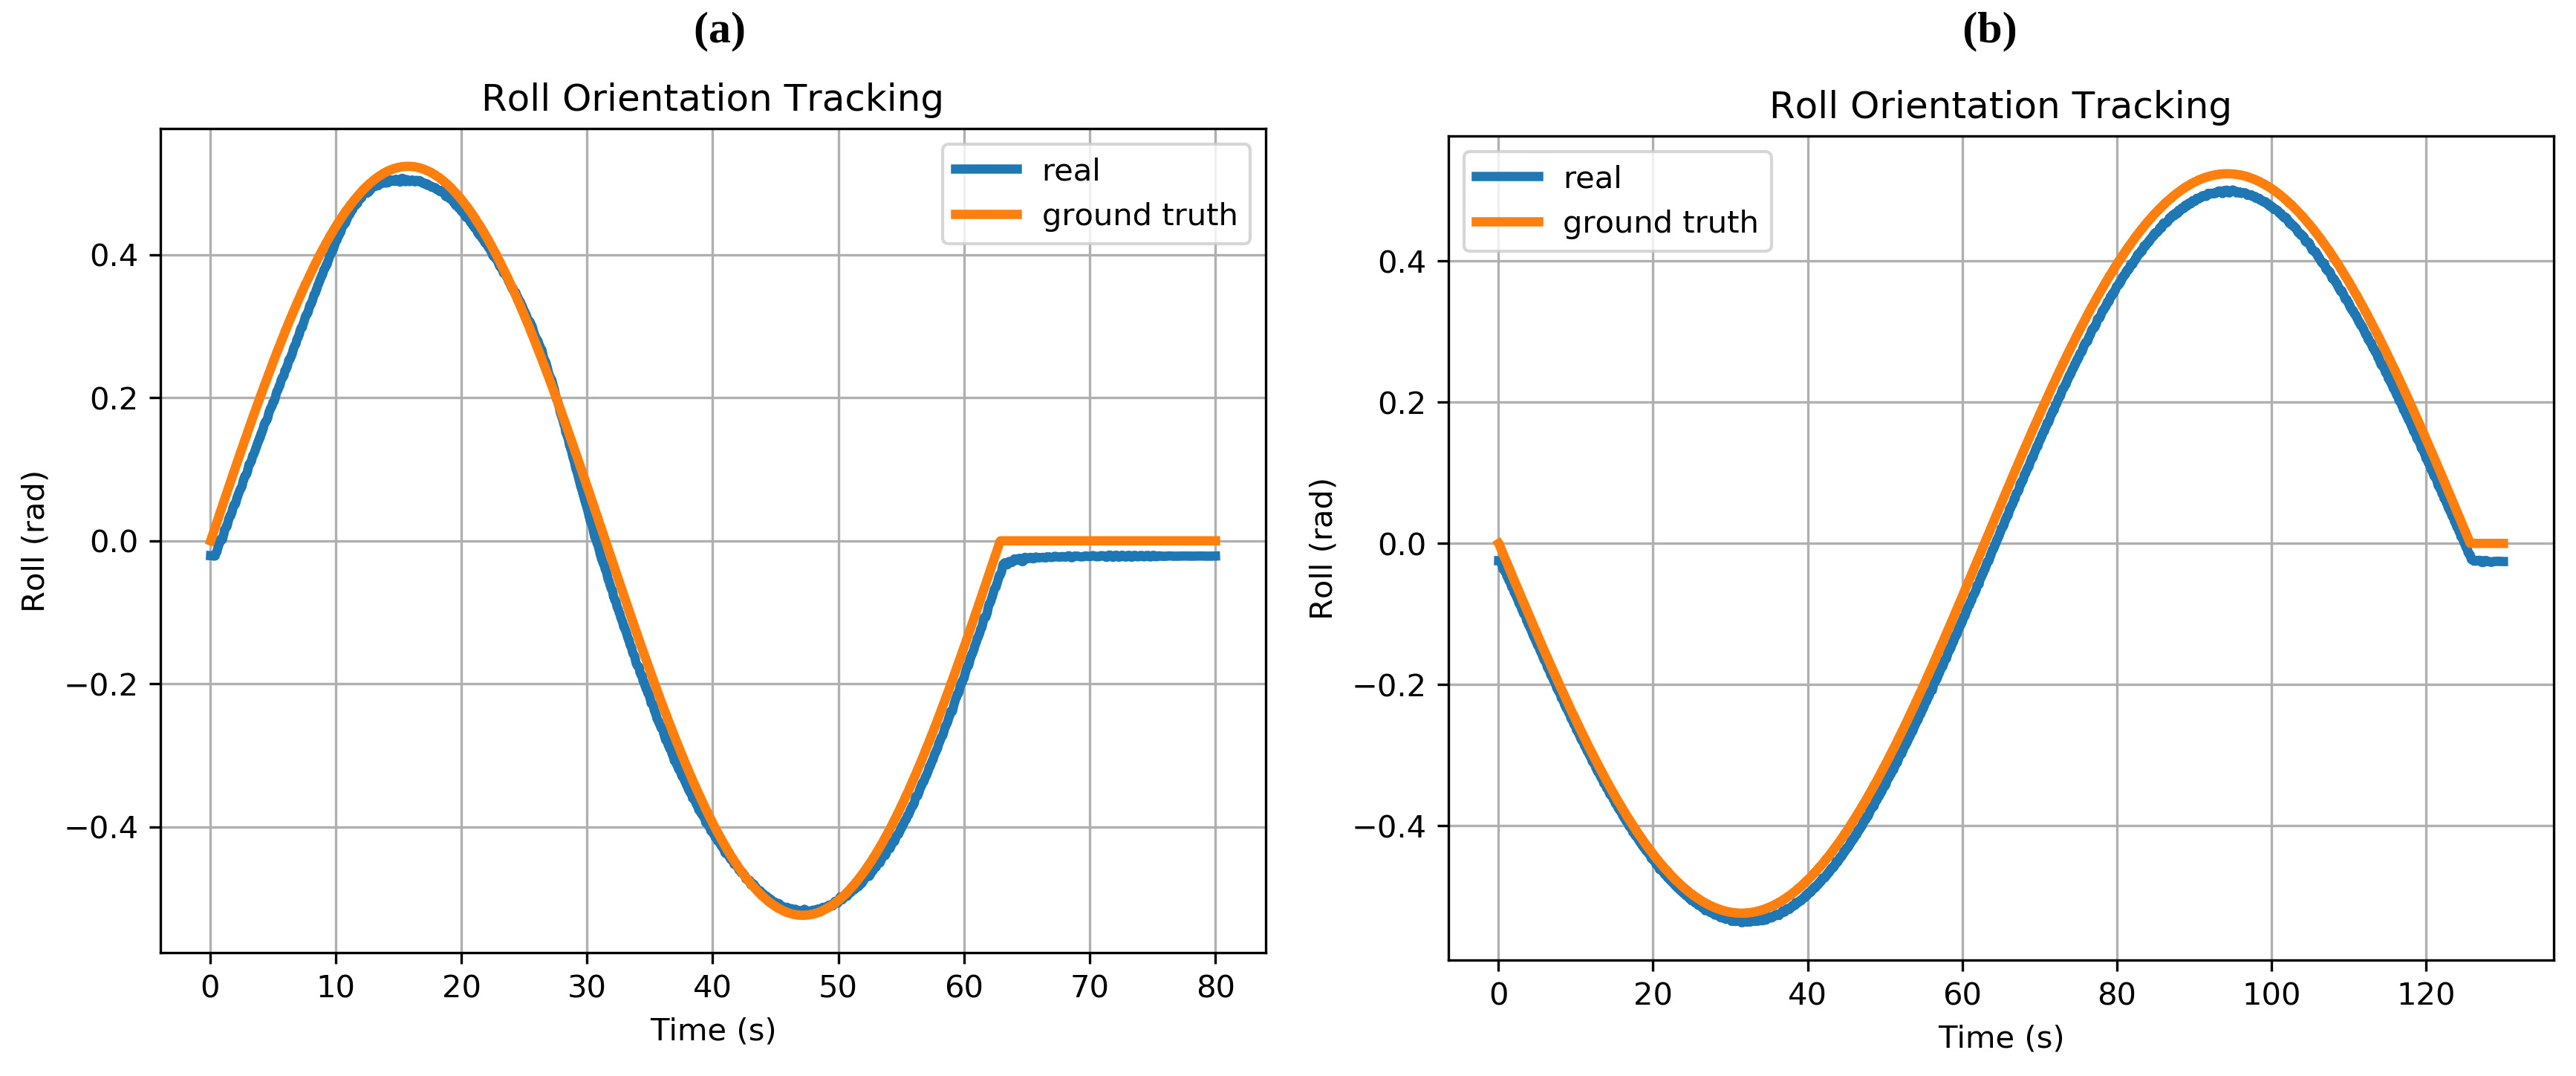
\includegraphics[width=\linewidth]{Fig_12.jpg}
%     \caption{Orientation variation about X-axis (a) 3-D Lissajous (b) Lemniscate}
%     \label{fig:orientation_varioation}
% \end{figure}
%%%%%%%%
\begin{table}[h]
\centering
\caption{Hardware performance on the Kinova Gen3 Lite: circle for all
four methods, plus PPO generalization to lemniscate, 3-D Lissajous, and
square without retraining. PPO is the only method that does not degrade
relative to its simulation result (Tab~\ref{tab:performance_comparison}). Best value per metric in
bold.}
\label{tab:trajectory_tracking}
\renewcommand{\arraystretch}{1.0}
\setlength{\tabcolsep}{3pt}
\begin{tabular}{llcc}
\toprule
\textbf{Method} & \textbf{Curve} & \textbf{Pos. RMSE} $\downarrow$ & \textbf{Orn. RMSE} $\downarrow$ \\
\midrule

Trac-IK
& Circle & 0.0362 & 0.0770 \\
\midrule

DLS
& Circle & 0.0490 & \textbf{0.0021} \\
\midrule

SAC
& Circle & 0.0450 & 0.0590 \\
\midrule

\multirow{3}{*}{PPO}
& Circle     & \textbf{0.0063} & 0.0320 \\
& Lemniscate & 0.0124 & 0.0212 \\
& Lissajous  & 0.0154 & 0.0410 \\

\bottomrule
\label{tab:error_metrics_real}
\end{tabular}
\end{table}
%%%%%%%%
% \begin{table}[h]
% \centering
% \caption{Real-Time Trajectory Tracking Performance on Hardware}
% \label{tab:error_metrics_real}
% \begin{tabular}{lccccc}
% \midrule
% \textbf{Trajectory} & \textbf{Pos RMSE(m)} & \textbf{Orn RMSE(rad)} \\
% \midrule\midrule
% Circle & $\boldsymbol{6.4\times 10^{-3}}$ & $3.4 \times 10^{-2}$ \\
% Lemniscate & $1.2\times 10^{-2}$ & $\boldsymbol{3.0 \times 10^{-2}}$\\
% 3-D Lissajous & $1.5\times 10^{-2}$ & $5.0 \times 10^{-2}$\\
% Square & $9.9\times 10^{-3}$ & $3.2 \times 10^{-2}$ \\
% \midrule
% \end{tabular}
% \end{table}

The sim-to-hardware transition reveals which methods rely on assumptions
that do not survive contact with real actuator dynamics. TRAC-IK's
position RMSE degrades by roughly 29$\times$ on hardware relative to
simulation (1.2~mm $\rightarrow$ 36.2~mm), the largest gap of any method.
This follows directly from its lack of a feedback term linking
consecutive solves: each waypoint is resolved independently from joint
encoder feedback with no mechanism to detect or correct accumulated
real-world drift, transmission backlash, or actuator lag between
solves, errors that do not exist in a noiseless simulation. DLS degrades
by a comparatively moderate $\sim$3$\times$ (16~mm $\rightarrow$ 49~mm),
consistent with its damping factor being calibrated against an idealized
simulated Jacobian that does not account for joint compliance and
backlash present on the physical Kinova Gen3 Lite; its orientation
advantage on the circle persists on hardware (2.1$\times10^{-3}$~rad,
still the best of any method), since the fixed-orientation condition that
produces this advantage in simulation is preserved on hardware. SAC
degrades by $\sim$1.5$\times$ (29~mm $\rightarrow$ 45~mm), consistent
with its sim-to-real gap being dominated by the same entropy-energy
equilibrium offset already present in simulation, rather than by an
additional hardware-specific failure mode.

PPO is the only method that does not degrade from simulation to
hardware: position RMSE on the circle is 6.3~mm on hardware against
9.95~mm in simulation. This is consistent with the additive Gaussian
perturbation noise injected at the policy output during training
(Eq.~\ref{noise}), which serves as implicit domain randomization, the policy is trained to remain accurate under actuator-level noise of comparable magnitude to what it encounters on hardware, so the sim-to-hardware transition does not expose an unmodeled failure mode the way it does for the purely kinematic and feedback-only classical baselines. Across all four hardware trajectories, PPO maintains position RMSE between 6.3~mm and 15.4~mm without retraining (Tab~\ref{tab:error_metrics_real}), with the lemniscate and 3-D Lissajous curves, which present orientation variation and curvature not
explicitly represented in the static-pose training distribution,
showing only a modest increase in error. This generalization is a direct
consequence of training on a dense, joint-limit-aware sample of the
reachable workspace pose-error space (Sec~\ref{simulation}) rather than on trajectory-specific demonstrations: since the policy's input is
instantaneous pose error rather than a trajectory index, any sufficiently
dense coverage of that error space at training time transfers to
trajectory geometries never seen during training.

Taken together, the simulation and hardware results support a single
consistent claim: the proposed reward structure, not the choice of PPO
as an optimizer, is responsible for the method's accuracy-smoothness
balance in simulation and its resistance to sim-to-real degradation on
hardware. Each classical baseline's hardware result degrades by an
amount that follows directly from a documented limitation of its control
structure, open-loop drift accumulation for TRAC-IK, fixed-gain
miscalibration for DLS, persistent entropy-driven offset for SAC, while
the proposed method's behavior on hardware is, within measurement
variation, predicted by its own training-time noise model.

% The trajectories tracked by Kinova Gen3 Lite end-effector, the circular trajectory Fig.~\ref{real_trajec_const_orientation}(a) achieves a position RMSE of 0.0064~m and an orientation RMSE of 0.0345~rad. The square trajectory Fig.~\ref{real_trajec_const_orientation}(b) demonstrates accurate corner navigation with position RMSE of 0.0099~m, guaranteeing the policy's ability to handle rapid direction changes through differential velocity commands without configuration-space discontinuities.

% Further, the 3-D Lissajous Fig.~\ref{real_trajec_var_orientation}(a) and lemniscate Fig.~\ref{real_trajec_var_orientation}(b) trajectories present geometrically complex scenarios with varying end-effector orientation as shown in Fig.\ref{fig:orientation_varioation}. These trajectory trackings exhibit slightly higher position RMSEs of 12.4~mm and 15.4~mm, respectively. The policy is trained on randomly distributed reachable poses in the robot's workspace, while these trajectories present requirements for high curvature, plane variations, and geometrically dense regions not explicitly presented during training time. Despite this, the policy tracks both the lemniscate and 3-D Lissajous continuously and stably without any re-training, demonstrating that the learned differential IK mapping generalizes zero-shot to complex trajectory geometries well beyond its training distribution. In addition, Fig.~\ref{fig:extra-real} illustrates the hardware deployment results for TRAC-IK, DLS, and SAC-S.


\section{CONCLUSIONS}
\label{conclusion}
This work presented a reactive, online differential inverse kinematics
controller for non-spherical wrist manipulators, in which a novel coupled
reward function, combining a min-operator pose reward (Eq.~\ref{final_pose_reward}), asymmetric
progress shaping (Eq.~\ref{progress_reward}), and an exponential energy penalty (Eq.~\ref{energy_penalty}),
constitutes the central contribution rather than the choice of reinforcement
learning algorithm. Operating on a compact 19-dimensional observation of
joint state and instantaneous pose error (Tab~\ref{tab:obs_action}), the policy requires no explicit Jacobian inversion, no online IK solve, and no trajectory-specific supervision, learning purely from joint-limit-aware static pose-reaching samples (Sec~\ref{simulation}) and generalizing zero-shot to circular, square, lemniscate, and 3-D Lissajous trajectory tracking at deployment.

The simulation and hardware results (Sec~\ref{results}) show that no single classical baseline is uniformly competitive across the evaluated metrics: TRAC-IK achieves the lowest position RMSE in simulation on planar curves but is three to four orders of magnitude less smooth than every other method and degrades most severely on hardware (Tab~\ref{tab:error_metrics_real}); DLS attains the best orientation tracking on the circle, but this advantage is specific
to constant-orientation motion and is lost on the lemniscate; and SAC
converges to a persistent offset driven by its entropy objective conflicting with the energy penalty. The proposed method does not achieve the lowest simulation error on every individual curve, but it is the only method whose position RMSE remains within a narrow band across all three simulated geometries, whose smoothness is the best of any method on every curve, and whose hardware performance does not degrade relative to simulation, in contrast to the classical baselines (Sec~\ref{real_time_deployment}). These properties follow directly from the structure of the proposed reward rather than from PPO as an optimizer, supporting the claim that the reward design, not the learning algorithm, is the mechanism responsible for the observed accuracy-smoothness-robustness trade-off.

The present framework has several limitations that bound the scope of
these claims. Hardware validation is restricted to a single manipulator,
the Kinova Gen3 Lite; generalization to other non-spherical wrist platforms
(such as KUKA, ABB, or UR variants with offset wrist axes) has not been
tested, and the cost of porting the policy to a different kinematic
structure is unknown. The policy was trained with a single random seed;
while the reported hardware and simulation results are consistent with the
training-time noise model (Eq.~\ref{noise}), the variance of this approach across independent training runs has not been characterized. Hardware baseline comparison was restricted to the circular trajectory for TRAC-IK, DLS, and SAC, while the proposed method was further validated on lemniscate, 3-D Lissajous, and square trajectories without retraining; a head-to-head hardware comparison on the geometrically more complex trajectories remains open. Controller behavior near kinematic singularities also remains uncharacterized: although the robot is initialized at the zero configuration at every episode reset, the policy has not been explicitly trained on singularity-proximal configurations, and its recovery behavior at kinematic boundaries is therefore implicit rather than verified. Finally, because the policy has no explicit dynamic model or closed-form stability guarantee, it does not offer the formal safety guarantees available to model-based controllers, a property that may matter for contact-rich or safety-critical deployment even though it is not required for the reactive, non-contact tracking tasks evaluated here.

Future work will address these limitations directly. Singularity-proximal
configurations will be incorporated during rollout collection to enable
verified recovery behavior at kinematic boundaries. Multi-seed training
will be used to quantify the variance of the proposed reward structure's
accuracy and smoothness advantages, and the hardware baseline comparison
will be extended to the non-circular trajectories. Validation on additional
non-spherical-wrist manipulators will be pursued to test whether the
consistency observed here is specific to the Kinova Gen3 Lite or a more
general property of the reward design. Finally, the framework will be
extended to dual-arm manipulation, where the learned differential IK
controller would serve as a per-arm low-level policy for coordinated
bi-manual control, a natural extension toward collaborative assembly
operations requiring simultaneous precise trajectory tracking under contact
constraints.

\section*{CRediT authorship contribution statement}
Surya Prakash S.K: Writing – original draft, Conceptualization, Validation, Methodology, Formal analysis, Software, Investigation, Visualization, Data curation. Sai Teja Majji: Writing – review and editing, Conceptualization, Validation, Methodology, Formal analysis, Software. Darshankumar Prajapati: Writing – review and editing, Conceptualization, Validation, Methodology. Jagannath Prasad Sahoo: Writing – review and editing, Visualization, Validation. Pushkar Kumar: Writing – review and editing, Visualization, Validation. Jayakumar V.K: Writing – review and editing, Visualization, Validation. Amit Shukla: Writing – review and editing, Supervision, Conceptualization, Funding acquisition.
\section*{Declaration of competing interest}
The authors declare that they have no known competing financial
interests or personal relationships that could have appeared to influence the work reported in this paper.
\section*{Data availability}
The source codes used in this work are in this \href{https://github.com/suryaroboticarm/Differential-Inverse-Kinematics-with-Coupled-Reward-Design}{git-hub} repository and the data used for training is available in this \href{https://drive.google.com/file/d/1BO6DrKE7GO-1D8vohWwWejpfg7DyryN8/view?usp=sharing}{drive}.



% \subsection{Example Subsection}
% \label{subsec1}

% Subsection text.

% %% Use \subsubsection, \paragraph, \subparagraph commands to 
% %% start 3rd, 4th and 5th level sections.
% %% Refer following link for more details.
% %% https://en.wikibooks.org/wiki/LaTeX/Document_Structure#Sectioning_commands

% \subsubsection{Mathematics}
% %% Inline mathematics is tagged between $ symbols.
% This is an example for the symbol $\alpha$ tagged as inline mathematics.

% %% Displayed equations can be tagged using various environments. 
% %% Single line equations can be tagged using the equation environment.
% \begin{equation}
% f(x) = (x+a)(x+b)
% \end{equation}

% %% Unnumbered equations are tagged using starred versions of the environment.
% %% amsmath package needs to be loaded for the starred version of equation environment.
% \begin{equation*}
% f(x) = (x+a)(x+b)
% \end{equation*}

% %% align or eqnarray environments can be used for multi line equations.
% %% & is used to mark alignment points in equations.
% %% \\ is used to end a row in a multiline equation.
% \begin{align}
%  f(x) &= (x+a)(x+b) \\
%       &= x^2 + (a+b)x + ab
% \end{align}

% \begin{eqnarray}
%  f(x) &=& (x+a)(x+b) \nonumber\\ %% If equation numbering is not needed for a row use \nonumber.
%       &=& x^2 + (a+b)x + ab
% \end{eqnarray}

% %% Unnumbered versions of align and eqnarray
% \begin{align*}
%  f(x) &= (x+a)(x+b) \\
%       &= x^2 + (a+b)x + ab
% \end{align*}

% \begin{eqnarray*}
%  f(x)&=& (x+a)(x+b) \\
%      &=& x^2 + (a+b)x + ab
% \end{eqnarray*}

% %% Refer following link for more details.
% %% https://en.wikibooks.org/wiki/LaTeX/Mathematics
% %% https://en.wikibooks.org/wiki/LaTeX/Advanced_Mathematics

% %% Use a table environment to create tables.
% %% Refer following link for more details.
% %% https://en.wikibooks.org/wiki/LaTeX/Tables
% \begin{table}[t]%% placement specifier
% %% Use tabular environment to tag the tabular data.
% %% https://en.wikibooks.org/wiki/LaTeX/Tables#The_tabular_environment
% \centering%% For centre alignment of tabular.
% \begin{tabular}{l c r}%% Table column specifiers
% %% Tabular cells are separated by &
%   1 & 2 & 3 \\ %% A tabular row ends with \\
%   4 & 5 & 6 \\
%   7 & 8 & 9 \\
% \end{tabular}
% %% Use \caption command for table caption and label.
% \caption{Table Caption}\label{fig1}
% \end{table}


% %% Use figure environment to create figures
% %% Refer following link for more details.
% %% https://en.wikibooks.org/wiki/LaTeX/Floats,_Figures_and_Captions
% \begin{figure}[t]%% placement specifier
% %% Use \includegraphics command to insert graphic files. Place graphics files in 
% %% working directory.
% \centering%% For centre alignment of image.
% \includegraphics{example-image-a}
% %% Use \caption command for figure caption and label.
% \caption{Figure Caption}\label{fig1}
% %% https://en.wikibooks.org/wiki/LaTeX/Importing_Graphics#Importing_external_graphics
% \end{figure}


% %% The Appendices part is started with the command \appendix;
% %% appendix sections are then done as normal sections
% \appendix
% \section{Example Appendix Section}
% \label{app1}



\bibliographystyle{elsarticle-num}
\bibliography{ref}

\end{document}
